%!TEX root = ../thesis.tex
%*******************************************************************************
%*********************************** Forecasting chapter *****************************
%*******************************************************************************

\chapter[Forecasting data requirements for \glsxtrshort{mpc}]{Data requirements of load forecasting for model predictive control} \label{chap:forecasting}

\graphicspath{{Forecasting/Figs/}}

\begin{cbox}{}
    \printpublication{langtry2024ImpactDataForecasting}

    \noindent{\color{black!50}\rule{\textwidth}{0.4mm}}\vspace{2mm}

    \noindent
    This chapter has been published as the journal article above. The co-authors of this article developed the code for the simple neural models used in the experiments. They also performed the data similarity metric and change-point analyses, detailed in Appendices \ref{app:forecasting-similarity-metric} \& \ref{app:forecasting-change-points}, and the data feature and online training experiments in Section \ref{sec:forecasting-data-efficiency}, providing a small amount of the text describing these analyses. Other than these contributions, all of the code, analysis, and text in this chapter is my own work.
\end{cbox}

\begin{cbox}{}
    All code and data used to perform the experiments in this chapter is available at \url{https://github.com/EECi/Annex_37}.
\end{cbox}

\hfill \\

%********************************** Graphical abstract **************************************
\begin{figure}[h]
    \centering
    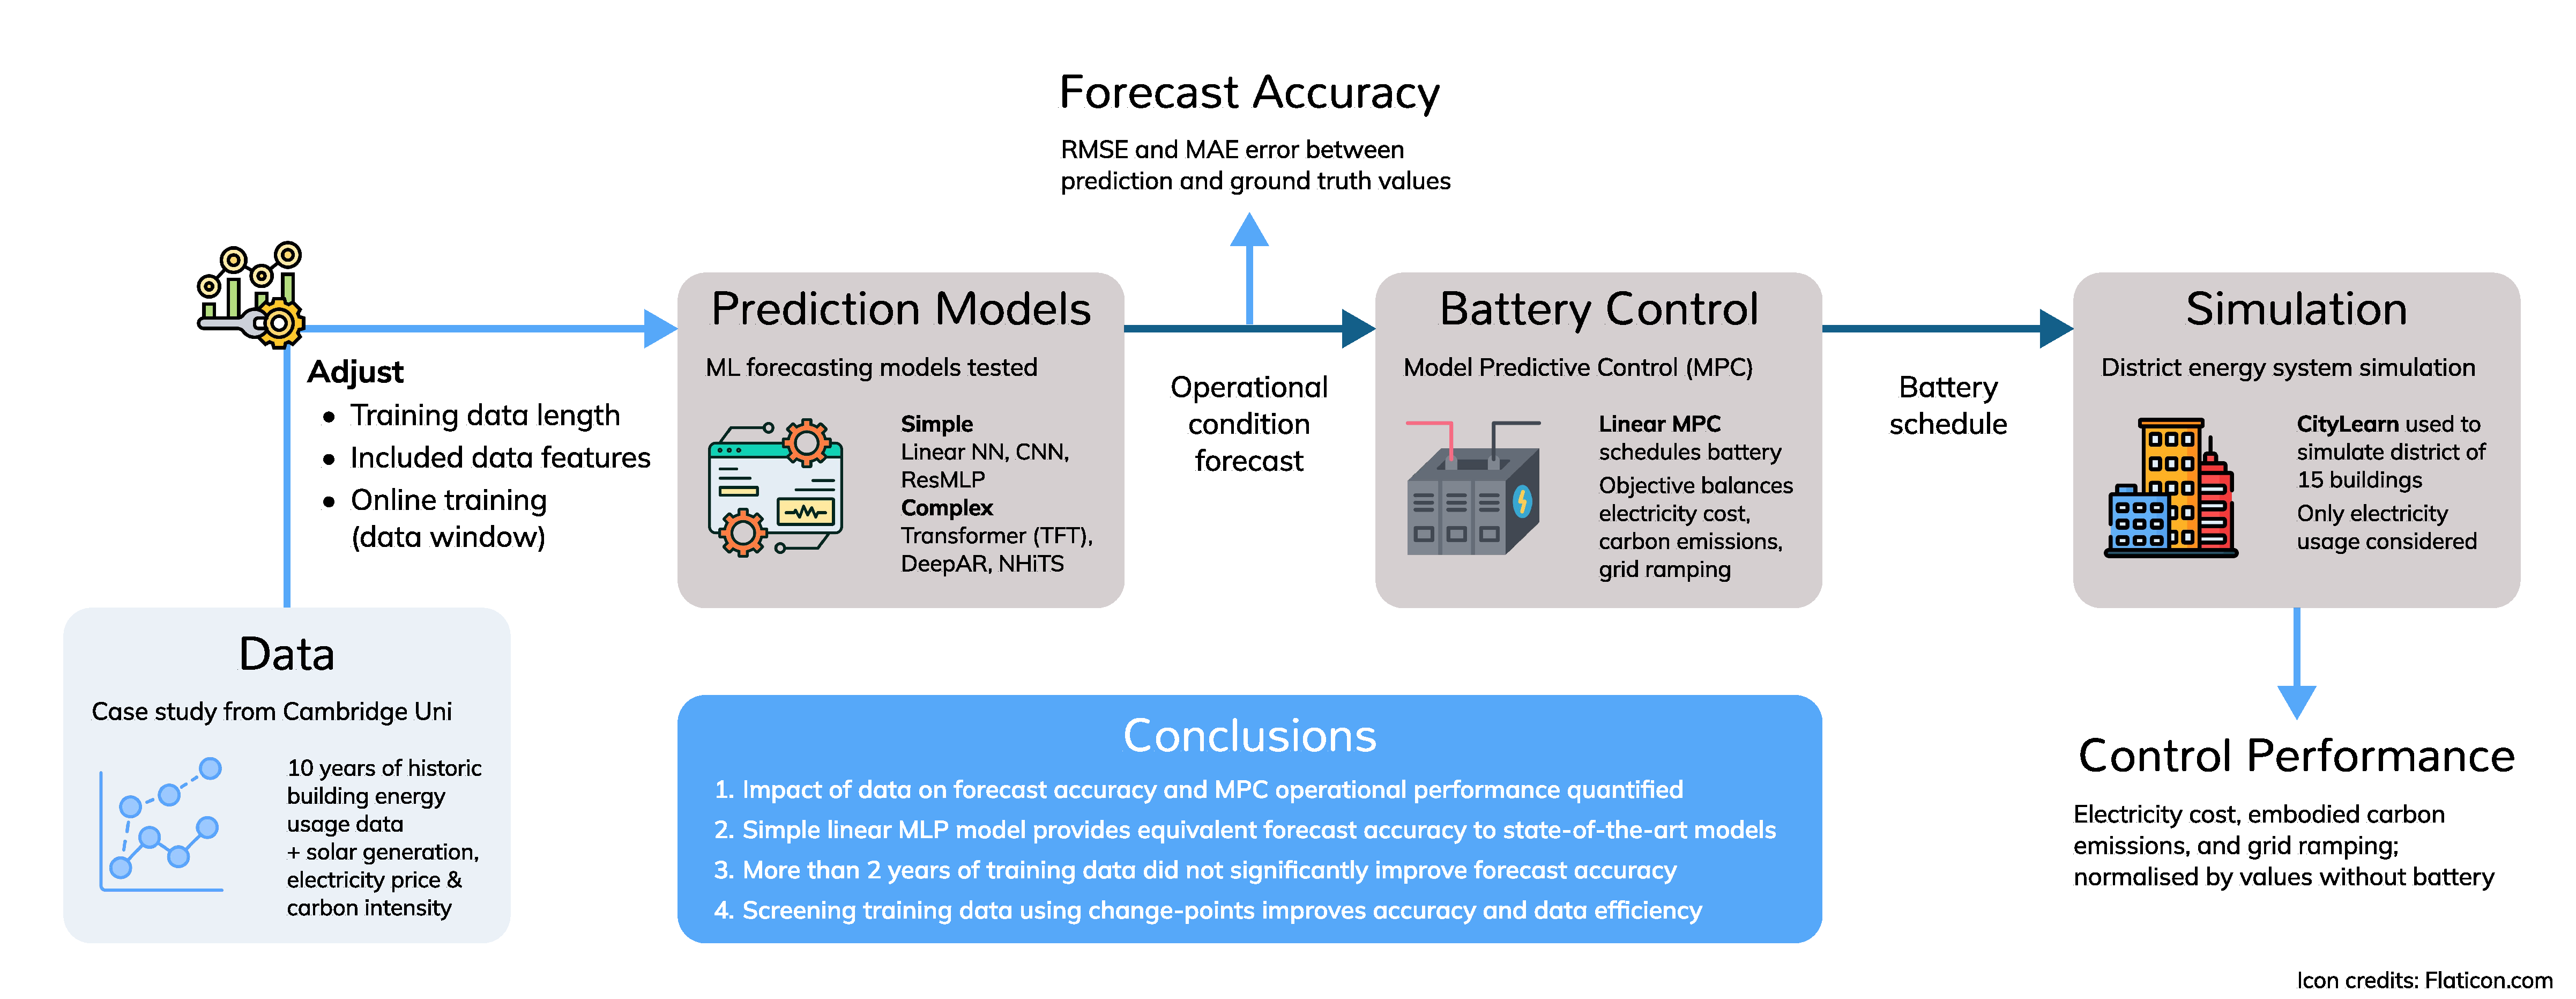
\includegraphics[width=\textwidth]{Graphical_Abstract.pdf}
    \caption{Graphical abstract of \Cref{chap:forecasting}.}
    \label{fig:forecasting-forecasting_graphical_abstract}
\end{figure}
\hfill \\
%********************************** end **************************************

\vspace{0.5cm}

\noindent
Data is needed to develop forecasting models for building behaviour that are used for smart control of the building energy systems to reduce the cost and carbon emissions of building operation. However, this data is costly to both collect and exploit. Determining the most cost effective data usage strategies and setting data collection requirements for these systems requires understanding of how data affects forecast accuracy, and the resulting impact on the operational performance of the building control. This chapter investigates how the available data affects the forecasting accuracy of machine learning prediction models, and how the accuracy of these prediction models affects the performance of \glsxtrlong{mpc} in a simulated multi-building energy system. The data requirements of state-of-the-art and simple textbook machine learning models are compared, and measures to improve the data efficiency of these models are investigated. Specifically, reuse of prediction models, reduction of training data duration, reduction of model data features, and online model training.


\newpage
%********************************** Intro section **************************************
\section{Introduction}

Distributed generation and storage technologies, most commonly solar panels and batteries, are used to reduce the cost and or operational emissions building energy systems \citep{aminitoosi2022BuildingDecarbonizationAssessing,oshaughnessey2021DemandSideOpportunityRoles,zhu2023ReviewDistributedEnergy}. `Smart' operation of these energy storage systems can reduce the impact the building's energy usage has on the electrical grid, by allowing energy flexibility through demand-side management and demand response \citep{vazquez-canteli2020MARLISAMultiAgentReinforcement}. This is particularly important in light of the expected electrification of heating demands \citep{leibowicz2018OptimalDecarbonizationPathways}, and the peak load issues this will cause. The effectiveness of these systems, quantified by operational performance metrics of the building energy system such as total electricity cost, incurred carbon emissions, and measures of grid impact, is determined by the ability of the storage control scheme to arbitrage energy and alter the timing of net energy usage to meet these operational goals. As a result, lots of research effort has been put into developing performant storage control strategies in recent years \citep{drgona2020AllYouNeed,wang2020ReinforcementLearningBuilding,kathirgamanathan2021DatadrivenPredictiveControl}.

\glsxtrlong{mpc} (\glsxtrshort{mpc}) is one of the two leading control methodologies in the current building energy systems literature, alongside \glsxtrlong{rl} (\glsxtrshort{rl}). Its use in smart energy storage systems in buildings has been widely studied \citep{zhou2021IncorporatingDeepLearning,deng2023EvaluationDeployingDatadriven,souto2018ScenarioBasedDecentralizedMPC,touretzky2014IntegratingSchedulingControl,lee2020ModelPredictiveControl}, and it has been found to provide substantial operational performance improvements compared to \glsxtrlong{rbc} (\glsxtrshort{rbc}) \citep{lee2020ModelPredictiveControl,erfani2021AnalysisImpactPredictive,oldewurtel2012UseModelPredictive}, the main technology used in existing building systems. It has also been shown to provide comparable performance to \glsxtrshort{rl} based control \citep{zhan2023ComparingModelPredictive}. Review papers \citep{wang2022ScienceMappingApproach,thieblemont2017PredictiveControlStrategies,farrokhifar2021ModelPredictiveControl} provide a thorough overview of the applications of \glsxtrshort{mpc} to building energy systems with distributed generation and storage.

\glsxtrshort{mpc} requires a model of the system dynamics, which estimates the next state of the system given; (a) the current system state, (b) current operational conditions, and (c) the applied control actions. Using this dynamics model and forecasts of the operational conditions over a given planning horizon, it predicts the operation of the system over that planning horizon. Optimization techniques are then used to determine the set of control actions that optimize a specified objective over the planning horizon. The performance of \glsxtrshort{mpc} therefore depends on: the accuracy of the system dynamics model, the accuracy of the operational condition forecasts, the ability of the optimization method to identify near-optimal control actions, and the match between the objective over the planning horizon and the global operational goals of energy management for the system. This chapter focuses on the accuracy of operational condition forecasts, and its resulting impact on the operational performance of \glsxtrshort{mpc}. \citep{raisch2025AdaptingChangeComparison} explores how data affects the accuracy of the system dynamics model, building on previous work on the topic by the main author \citep{raisch2025GenTLGeneralTransfer}.


\subsection{Forecasting models for \glsxtrshort{mpc}}

Lots of different time series forecasting methodologies have been studied for the predicting operational conditions for building energy management \citep{sun2020ReviewThestateoftheartDatadriven}, however recent research has focused on machine learning based methods \citep{zhang2021ReviewMachineLearning,chou2018ForecastingEnergyConsumption,dai2023ComparisonDifferentDeep,rahman2018PredictingElectricityConsumption,fan2019AssessmentDeepRecurrent} due to their promising performance. Successes in other fields have prompted the investigation of large-scale, high-complexity model architectures \citep{choi2023PerformanceEvaluationDeep,dai2023CityTFTTemporalFusion}. However, there is doubt about whether such complex models are appropriate for use in the context of \glsxtrshort{mpc} for building energy systems \citep{zeng2023AreTransformersEffective,bunning2022PhysicsinformedLinearRegression,bunning2021ComparingMachineLearning}, due to the computational and data availability limitations in practical systems. So both simple and high-complexity, state-of-the-art machine learning forecasting models are investigated.


\subsection{Impact of data on forecast accuracy and \glsxtrshort{mpc} performance}

As machine learning methods are purely data-driven, `black box' prediction models, achieving accurate forecasts requires the availability of training data that is representative of the building energy system for which the model will be used. However, acquiring representative training data is both challenging and costly.
The costs of acquiring data include not only the capital costs of installing monitoring systems, but also the costs of digital infrastructure, data processing, system maintenance, and quality assurance required to support data collection. For the case of developing forecasting models for \glsxtrshort{mpc} considered in this study, there are additional project costs associated with delaying the installation of the battery system while data is gathered. \citep{motegi2003CaseStudiesEnergy} estimates the capital cost of electricity and gas smart-metering for a university campus to be \$0.27/m$^2$, plus an additional \$0.11/m$^2$ for maintenance and supporting IT systems. However, this considers only the cost of collecting data, and neglects the significant costs of training and deploying machine learning models \citep{strubell2020EnergyPolicyConsiderations}, from both the computing and expertise required.
Whilst the importance of data availability and the impact of data on forecast accuracy are widely acknowledged in the existing literature \citep{kathirgamanathan2021DatadrivenPredictiveControl,lee2020ModelPredictiveControl,wang2022ScienceMappingApproach,choi2023PerformanceEvaluationDeep,zhan2021DataRequirementsPerformance}, few works study the role of data in enabling good operational performance for \glsxtrshort{mpc} in building energy systems.

Determining cost optimal data collection strategies to support the development of forecasting models for \glsxtrshort{mpc} in buildings requires understanding of the trade-off between the quantity of data \& data features used for model training, and its associated costs, and the operational performance achieved by the controller. This impact of data for forecasting on \glsxtrshort{mpc} operational performance can be considered in two stages, by firstly studying the relationship between data and forecast accuracy of the resulting models, and then the sensitivity of the controller operational performance to the accuracy of forecasts.\\

Only a single previous study has investigated the impact of data on the accuracy of forecasting models for building energy management. This work, \citep{choi2023PerformanceEvaluationDeep}, compares the prediction accuracy of deep learning architectures for forecasting thermal loads and building zone temperatures over varying training dataset sizes. It finds that increasing the training data length does not always improve prediction accuracy due to the strong seasonality of building energy behaviours, but that the addition of data with good similarity to the test dataset into the training dataset greatly improves forecast accuracy. A limitation of this study is that it analyses only a single year of thermal load and zone temperature data, synthesised from a building energy model and historical weather data, meaning that a limited range of training dataset sizes, from 3 to 9 months, is considered. As a result, training data preceding the test data by one year, which due to seasonality is likely to have the highest similarity and so greatest value, is unavailable, meaning the study of the benefit of additional training data is incomplete.\\

The impact of forecast accuracy on \glsxtrshort{mpc} operational performance has been studied to a limited extent. \citep{erfani2021AnalysisImpactPredictive} compares the use of various classical and machine learning forecasting models in a common \glsxtrshort{mpc} framework, quantifying both the forecast accuracy and resulting operational performance of \glsxtrshort{mpc}. However, the models studied all achieve comparable forecast accuracies and operational performances, meaning limited insight can be gained into the relationship between the two. Further, as comparison is made between model types, these results cannot be used to assess the benefit of forecast improvement for any individual model.
\citep{oldewurtel2012UseModelPredictive} shows that the use of more accurate, external weather forecasts improves \glsxtrshort{mpc} operational performance, but does not quantify the forecast accuracies for comparison. In \citep{bartolucci2019HybridRenewableEnergy}, the prediction accuracy and corresponding operational performance of \glsxtrshort{mpc} for two forecasts of electrical load with different levels of synthetic noise are quantified. Finally, \citep{enriquez2016SolarForecastingRequirements} provides the most complete study, investigating the variation of operational performance with the noise amplitude of synthetic forecasts of temperature and solar irradiance. However, as the forecast accuracy of the synthetic predictions is not quantified, these results cannot be compared to the performance of practical prediction models and used to assess the benefits of forecast accuracy improvements.

The direct impact of training data length on operational performance is studied in \citep{savadkoohi2023FacilitatingImplementationNeural}. It computes the operational performance achieved by a neural network based building thermal controller as the size of the training dataset varies, and finds that negligible performance improvements are obtained when using more than 8 months of training data. Whilst a comprehensive quantification of the relationship between training data volume and operational performance achieved by the specific control scheme studied is provided, the results are specific to the atypical controller architecture used, which does not include the explicit forecasting of operational variables used in typical \glsxtrshort{mpc} schemes. Additionally, other aspects of data, such as the inclusion of additional data variables, and the reuse of data from existing buildings, are not considered.\\

Questions of the impact of data on \glsxtrshort{mpc} performance in buildings, and the optimal data collection strategies to support model development, have been explored in the System Identification field \citep{zhan2021DataRequirementsPerformance,balali2023EnergyModellingControl,zhang2023InvestigationsMachineLearningbased,erfani2023LinkingDatasetQuality,zhan2022ImpactOccupantRelated,zhan2022ModelcentricDatacentricPractical} in the context of developing accurate system dynamics models for \glsxtrshort{mpc}, termed `control-oriented models'. Studies have investigated the data requirements of different modelling approaches \citep{zhan2021DataRequirementsPerformance,balali2023EnergyModellingControl,zhang2023InvestigationsMachineLearningbased}, the impact of data resolution on model accuracy \citep{erfani2023LinkingDatasetQuality}, the impact of model prediction accuracy on operational performance \citep{zhan2022ImpactOccupantRelated}, and cost optimal data collection strategies to support model development \citep{zhan2022ModelcentricDatacentricPractical}.


\newpage
\subsection{Research objectives \& contributions}

There has been very limited study of the impact of data on the prediction accuracy of forecasting models for building energy management. Additionally, there has been no study of the trade-off between the quantity of data \& data features used for model training, and the operational performance of \glsxtrshort{mpc} for battery scheduling in systems with distributed generation and storage. Understanding of this trade-off is necessary to properly prioritise expenditure on data collection for smart energy storage systems.
This chapter addresses this research gap by quantifying the impacts of data on both the prediction accuracy and operational performance of \glsxtrshort{mpc} using simple and high-complexity, state-of-the-art machine learning based prediction models. A simulated multi-building energy system with distributed solar generation and battery storage using historic building load measurement data is used as a case study. The main research objectives are to:
\begin{itemize}
    \itemsep0em 
    \item Compare the performance of simple and state-of-the-art machine learning models with regards to prediction accuracy, model generalisation, and data efficiency;
    \item Investigate the trade-off between data and forecast accuracy for the following data efficiency measures: reuse of prediction models, reduction of training data durations, reduction of model data features, and online model training;
    \item Propose strategies for improving prediction performance when selecting models for reuse and selecting data to exclude when reducing training data durations; and
    \item Quantify the relationship between forecast accuracy and resulting operational performance of \glsxtrshort{mpc}.
\end{itemize}
\hfill \\

The key research contribution is the combined study of the impact of data on both forecast accuracy and the resulting operational performance of \glsxtrshort{mpc}. This is important as it allows energy system designers to assess the trade-off between the cost of data for forecasting and the operational benefits it provides. The impact of aspects of data on forecast accuracy not yet studied in the context of building energy management are also investigated, specifically the reuse of prediction models, selection of model data features, and online model training. Two strategies for improving the efficacy of collected data for building load forecasting are proposed: a load profile similarity metric for selecting prediction models for reuse, and a change-point detection based methodology for screening training data to improve prediction performance whilst reducing model training time. Further, a long duration (10 year) historic building energy dataset is used to conduct these experiments, allowing performance to be evaluated on a multi-year scenario, providing more robust testing than existing studies.

The remainder of this chapter is structured as follows. Section \ref{sec:forecasting-experiment} describes the simulation framework and data used to perform the experiments, as well as the models tested, and how their performance is evaluated. In Section \ref{sec:forecasting-baseline-comparison}, the forecast accuracy of the prediction models trained without data duration limitations is evaluated to provide a baseline, and model performance is compared. Model generalisation for load prediction between buildings is then tested in Section \ref{sec:forecasting-generalisation}, to assess whether model reuse is a viable strategy for reducing data collection requirements for new smart energy storage systems. A load profile similarity metric based on the Wasserstein distance between functional Principal Component Analysis (fPCA) coefficient distributions is proposed, and its efficacy as a criterion for selecting models for reuse is tested. Section \ref{sec:forecasting-data-efficiency} studies the impact of various aspects of data on forecasting accuracy. The effect of the volume of data used for model training is studied in Section \ref{sec:forecasting-data-efficiency-training-data} to support decision making on the quantity of data that should be collected for model development. A change-point detection based methodology for screening training data is proposed, and its ability to improve prediction accuracy whilst reducing training data durations is investigated. The selection of model data features and use of online model training are considered in Sections \ref{sec:forecasting-data-efficiency-data-features} and \ref{sec:forecasting-online-training} respectively. Section \ref{sec:forecasting-control-sensitivity} contextualises the study of model forecast accuracy in the building energy system control task by quantifying the relationship between forecast accuracy and the resulting \glsxtrshort{mpc} operational performance for synthetic noisy forecasts. Finally, conclusions are drawn in Section \ref{sec:forecasting-conclusions}.


\newpage
%********************************** Experiments section **************************************
\section{Experimental setup} \label{sec:forecasting-experiment}

% ... to study benefit of data usage on forecasting for control, test MPC task is studied to provide context - aim of using data is to achieve improved operational performance - outline context, task, and models studied ...

\subsection{Smart building control simulation framework}

% Describe CityLearn \citep{vazquez-canteli2019CityLearnV1OpenAI,vazquez-canteli2020CityLearnStandardizingResearch} simulation + MPC control framework, as well as data variables within environment.

To study the impacts of data on forecasting and \glsxtrshort{mpc} performance in the context of building energy systems, a case study of an example multi-building building energy system was simulated. In this case study, \glsxtrshort{mpc} is used to schedule battery storage operation in the multi-building energy system containing distributed storage and solar generation, as to reduce the electricity price, carbon emissions, and grid impact associated with meeting the electrical demand of the buildings. The CityLearn \citep{vazquez-canteli2019CityLearnV1OpenAI,vazquez-canteli2020CityLearnStandardizingResearch} building energy control framework is used to simulate the behaviour of the building energy system, and provide the required data to a Linear Program based \glsxtrshort{mpc} implementation. A schematic of the energy flows within the simulated multi-building energy system is provided in Fig. \ref{fig:forecasting-energy-system}.

During simulations, at each time step, the prediction models use observation data to produce forecasts of the operational variables, which are passed to a linear predictive control model. The resulting linear optimisation problem is solved to determine the optimal control actions, which are then applied to the battery units in the CityLearn simulation. The combination of prediction models and linear predictive control model comprise the Linear \glsxtrshort{mpc} controller.
This simulation and control loop is illustrated in Fig. \ref{fig:forecasting-control-loop}.\\

\begin{figure}[h]
    \centering
    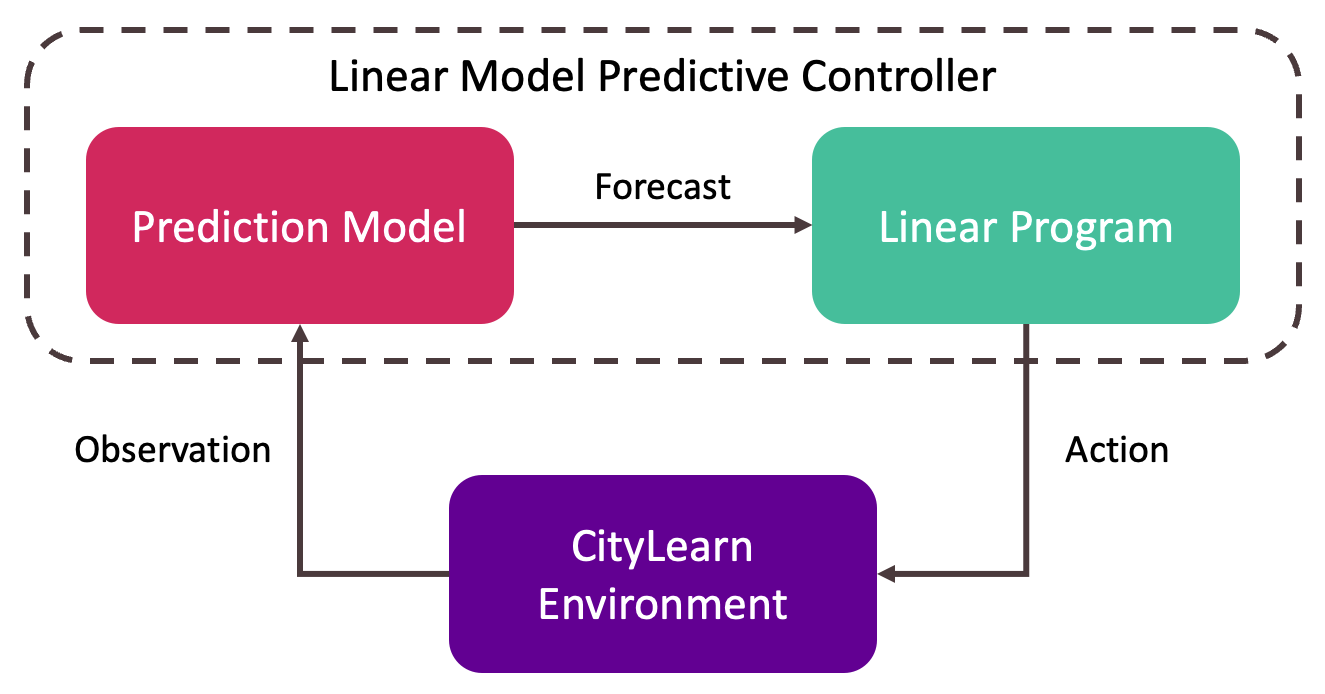
\includegraphics[width=0.66\textwidth]{Task/control-loop.png}
    \caption{Control loop for  test district-level building energy system simulation.}
    \label{fig:forecasting-control-loop}
\end{figure}

\newpage
The Linear Program formulation used in the \glsxtrshort{mpc} scheme is described by Eq. \ref{eq:forecasting-LP-example}, with Table \ref{tab:forecasting-LP-params} providing descriptions of the parameters. At each time step the optimised control actions, ${E_i}^*[\tau{=}0]$, are taken. The optimisation objective is comprised of three weighted components, which correspond to the cost of grid electricity consumed by the buildings (assuming no net electricity metering), the embodied carbon emissions associated with the grid electricity, and the ramping of the overall grid electrical demand which represents the grid impact. The three components are normalised by the values they would have if no battery storage were present in the buildings, denoted by $\widetilde{O}^k$ for component $k$, lower bounded at 1. This clipping is performed to prevent ill-conditioning of the objective when the no-storage objective values are small.

% Note that MPC system model is exact (designed for perfect match between simulator and controller), so only noise is from predictions (isolates impact) - we can get this because we are studying solar-battery systems (no heat), so say this is a reason why we chose a solar-battery system (electrical physics easy).

The CityLearn simulations are configured so that the building energy system has linear dynamics, which is possible as a solar-battery system is studied and only electrical behaviour is considered. As the system parameters are known to the controller, the \glsxtrshort{mpc} has a perfect model of the true system dynamics. This perfect match between the simulator and controller dynamics models means no inaccuracies are introduced in system identification. The optimality guarantees of Linear Programming, and the use of the global operational objective as the \glsxtrshort{mpc} objective, with sufficiently large planning horizon $T$, mean there is negligible distortion of the operational performance from these factors. This allows the effect of operational condition forecast accuracy on \glsxtrshort{mpc} operational performance to be studied in isolation - i.e. to a good approximation, sub-optimality in operational performance in the simulation environment is caused solely by forecasting inaccuracies.\\

\begin{figure}[h]
    \centering
    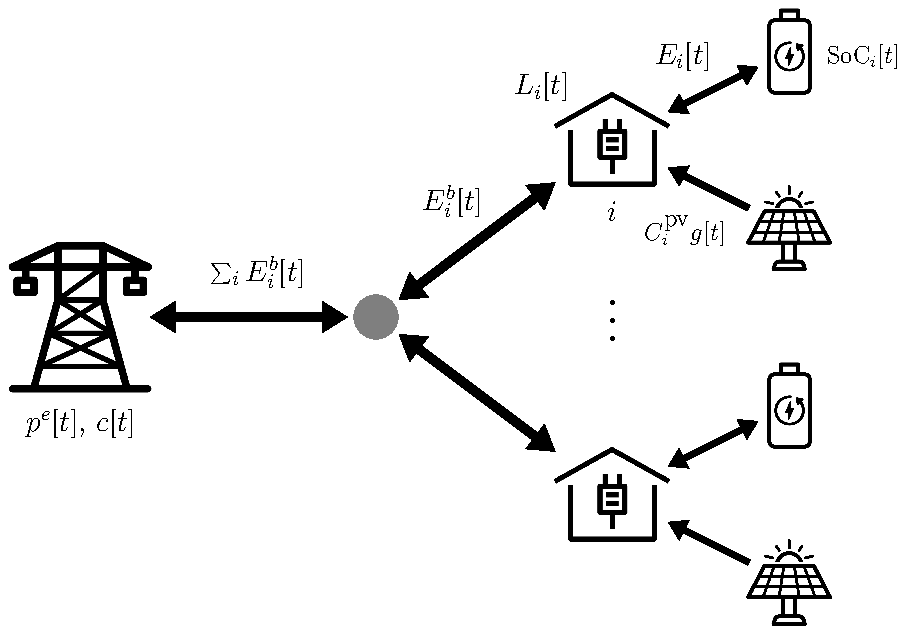
\includegraphics[width=0.7\linewidth]{Task/sys-diagram.pdf}
    \caption{Energy flow schematic for test multi-building energy system. {\small(Icon credits: \href{https://thenounproject.com/symbolon/}{Symbolon})}}
    \label{fig:forecasting-energy-system}
\end{figure}

\newpage
\begin{subequations} \label{eq:forecasting-LP-example}
    \begin{align}
        \addtocounter{equation}{-1}
        \begin{split}
        \text{min} & \qquad \frac{\gamma^p \,\, \mathlarger{\sum}_{\tau} \,\, p^e[t{+}\tau] \, \mathlarger{\sum_i} \left( \max \left[ 0,\, E_i^b[t{+}\tau] \right] \right)}{\raisebox{-1.2ex}{$\max \left[ 1, \widetilde{O}^p \right]$}} \\[1em]
        & \qquad\qquad + \,\, \frac{\gamma^c \,\, \mathlarger{\sum}_{\tau} \,\, c[t{+}\tau] \, \mathlarger{\sum_i} \left( \max \left[ 0,\, E_i^b[t{+}\tau] \right] \right)}{\raisebox{-1.2ex}{$\max \left[ 1, \widetilde{O}^c \right]$}} \\[1em]
        & \qquad\qquad\qquad\qquad + \,\, \frac{\gamma^r \,\, \mathlarger{\sum}_{\tau} \,\, \abs{\bigg( \mathlarger{\sum_i} \, E_i^b[t{+}\tau] \bigg) - \bigg( \mathlarger{\sum_i} \, E_i^b[t{+}\tau{-}1] \bigg)} }{\raisebox{-1.2ex}{$\max \left[ 1, \widetilde{O}^r \right]$}}
        \end{split} \label{eq:forecasting-lp} \\[1ex]
        \text{over} & \qquad E_i[\tau] , \, \textrm{SoC}_i[\tau{+}1] \quad \forall \: i,\, \tau \tag*{} \\
        \text{subject to} & \qquad \textrm{SoC}_i[\tau{+}1] \leq \textrm{SoC}_i[\tau] + \min\left[ E_i[\tau] \sqrt{\eta_i},\, E_i[\tau]/\sqrt{\eta_i} \right] \label{eq:forecasting-dynamics-constraint} \\
        & \qquad -P^{\textrm{max}}_i \Delta t \leq E_i[\tau] \leq P^{\textrm{max}}_i \Delta t \label{eq:forecasting-power-constraint} \\
        & \qquad 0 \leq \textrm{SoC}_i[\tau{+}1] \leq C^s_i \label{eq:forecasting-energy-constraint} \\
        & \qquad \textrm{SoC}_i[\tau{=}0] = \textrm{SoC}_i^t \label{eq:forecasting-initial-conditions} \\
        & \qquad E^b_i[\tau] = L_i[\tau] - C^{\textrm{pv}}_i g[\tau] + E_i[\tau] \label{eq:forecasting-aggregation-constraint} \\
        \text{for all} & \qquad i \in [0,B{-}1], \: \tau \in [0,T{-}1] \tag*{}
        % \text{apply actions} & \qquad E_i[\tau{=}0] \quad \forall \: i \tag*{}
    \end{align}
\end{subequations}

\newpage
\begin{table}[h]
    \centering
    \renewcommand{\arraystretch}{1.25}
    \begin{tabularx}{\linewidth}{ccX} \toprule \toprule
        Parameter & Units & \multicolumn{1}{>{\centering\arraybackslash}c}{Description} \\
        \midrule \midrule
        \multicolumn{3}{>{\centering\arraybackslash}l}{\small\it \quad Decision variables} \\
        $E_i[\tau]$ & kWh & Energy \textit{intake} to battery unit in building $i$ at time $\tau$ in planning horizon \\
        $\textrm{SoC}_i[\tau]$ & kWh & State-of-charge of battery unit in building $i$ at time $\tau$ in planning horizon \\
        \midrule
        \multicolumn{3}{>{\centering\arraybackslash}l}{\small\it \quad Data variables} \\
        $\Delta t$ & hrs & Time step of simulation data \\
        $C^s_i$ & kWh & Energy capacity of battery unit in building $i$ \\
        $C^{\textrm{pv}}_i$ & kWp & Peak power capacity of solar PV unit in building $i$ \\
        $\eta_i$ & -- & Round-trip efficiency of battery unit in building $i$ \\
        $P^{\textrm{max}}_i$ & kW & Power capacity of battery unit in building $i$ \\
        $\textrm{SoC}_i^t$ & kWh &  State-of-charge of battery unit in building $i$ at time $t$ \\
        $L_i[t]$ & kWh & Electrical demand of building $i$ at time $t$ \\
        $g[t]$ & kW/kWp & Normalised generation power from solar PV at time $t$ \\
        $p^e[t]$ & £/kWh & Grid electricity price at time $t$ \\
        $c[t]$ & kgCO$_2$/kWh & Carbon intensity of grid electricity at time $t$ \\
        $\gamma^p$ & -- & Fraction of objective from electricity cost component \\
        $\gamma^c$ & -- & Fraction of objective from CO$_2$ emissions component \\
        $\gamma^r$ & -- & Fraction of objective from grid ramping component \\
        \bottomrule \bottomrule
    \end{tabularx}
    \smallskip
    \caption{Description of Linear Program model parameters.} \label{tab:forecasting-LP-params}
\end{table}


\clearpage
\subsection{Forecasting task \& performance evaluation}

% Explicitly define the prediction task and explain accuracy metrics used to compare forecast qualities and that control performance is also used as it grounds prediction task in context

For the \glsxtrshort{mpc} scheme used, Eq. \ref{eq:forecasting-LP-example}, forecasts of the following operational condition variables over the planning horizon $T$ are required at each time instance, $t$:
\begin{itemize}
    \item electrical demand for each building, $L_i[t]$
    \item normalised solar PV generation power, $g[t]$
    \item price of grid electricity, $p^e[t]$
    \item carbon intensity of grid electricity, $c[t]$
\end{itemize}

This study investigates the impacts of data on the forecasting of these 4 types of operational variables. The accuracies of these forecasts are quantified using two error metrics, the normalised Mean Absolute Error (nMAE), and the normalised Root Mean Squared Error (nRMSE), given by Eqns \ref{eq:forecasting-nMAE} \& \ref{eq:forecasting-nRMSE},

\vspace*{0.5cm}
\begin{minipage}{0.5\linewidth}
\begin{equation} \label{eq:forecasting-nMAE}
    \frac{\frac{1}{N} \mathlarger{\sum_{t=0}^{N-1}} \, \frac{1}{T} \sum_{\tau=1}^{T} \abs{f^v_{t,\tau} - v_{t+\tau} } }{\frac{1}{N} \sum_{t=0}^{N-1} v_t}
\end{equation}
\end{minipage}%
\begin{minipage}{0.5\linewidth}
\begin{equation} \label{eq:forecasting-nRMSE}
    \frac{\frac{1}{N} \mathlarger{\sum_{t=0}^{N-1}} \sqrt{ \frac{1}{T} \sum_{\tau=1}^{T} \left(f^v_{t,\tau} - v_{t+\tau} \right)^2 } }{\frac{1}{N} \sum_{t=0}^{N-1} v_t}
\end{equation}
\end{minipage}
\vspace*{0.5cm}

where $f^v_{t,\tau}$ is the forecast of variable $v$ at time $t$ for time instance $\tau$ in the planning horizon, and $v_{t+\tau}$ is the true value of the target variable at time instance $t+\tau$. These error metrics are the means of the standard MAE and RMSE errors over all forecasting horizons considered in the simulation, normalised by the mean level of the target variables to allow comparability between forecast accuracies.

The operational performance achieved by the \glsxtrshort{mpc} scheme using a given set of prediction models is quantified by evaluating the objective specified in Eq. \ref{eq:forecasting-LP-example} with the simulated behaviour of the building energy system resulting from the use of the controller.

All experiments conducted in this study test the same multi-building energy system, with distributed energy assets as specified in Appendix \ref{app:forecasting-system-spec}, and use a planning horizon of $T=48$hrs, justification of this value is provided in Appendix \ref{app:forecasting-tau}, along with objective component weights, $(\gamma^p,\gamma^c,\gamma^r) = (0.45,0.45,0.1)$, in both the \glsxtrshort{mpc} scheme and for operational performance evaluation.


\newpage
\subsection{Building electricity usage data}

Historic building electricity metering data from the Cambridge University Estates dataset \citep{langtry2024CambridgeUniversityEstates}, described in Appendix \ref{app:data}, is used to provide a case study for the multi-building energy system. A 10 year period from 2010 to 2019 is chosen for the case study, so that data durations up to a maximum practical length can be tested. 15 buildings\footnote{The number of buildings that can be used in the study is limited by the computational cost of the forecasting methods and the system simulations.} with complete data availability for electrical load over this period are selected\footnote{Version 1 building numbers: 0, 3, 9, 11, 12, 15, 16, 25, 26, 32, 38, 44, 45, 48, 49} for use in the experiments, such that they cover a wide range of building scales and provide a good mix of similarity and dissimilarity with respect to their electricity loads.

Alongside the building electrical load data, which is assumed not to contain any significant contributions from space heating or cooling, the following other data variables are retrieved from the dataset: weather data for Cambridge (including outdoor temperature, relative humidity, and direct \& diffuse solar irradiance), local solar generation power, grid electricity price \& carbon intensity data, and temporal information (including hour, day, month indices, and daylight savings status).

The 10 years of data is initially split into training, validation, and test datasets covering the following periods: train (2010 to 2015), validate (2016 to 2017), test (2018 to 2019). For all experiments the test data is kept the same, however the periods of data used to train the prediction models are altered in Section \ref{sec:forecasting-data-efficiency}.

\subsection{Brief description of the prediction models}

% Briefly outline models studied. We pit simple models against SOTA. Offload technical details to \ref{app:forecasting-models}.

Data and computational requirements, which vary across predictions models, are important considerations for the deployment of \glsxtrshort{mpc} based controllers in practical building energy systems. This work investigates the performance of 6 machine learning based prediction models which span a range of model characteristics; 3 simple neural models, and 3 high-complexity, state-of-the-art models. A brief description of each model architecture follows. Technical specifications of the model implementations used are provided in Appendix \ref{app:forecasting-models}.

\subsubsection{Simple neural models}

Recent literature, \citep{zeng2023AreTransformersEffective}, has shown that simple neural models using Direct Multi-Step forecasting (DMS), where all predictions over the forecast window are generated concurrently, can outperform complex, transformer-based models using traditional, Iterated Multi-Step forecasting (IMS), in which a single-step forecaster is applied iteratively to generate a multi-step forecast. For all three simple neural architectures investigated, DMS forecasting is used.

\paragraph{Linear neural network (Linear)}

A Multi-Layer Perceptron (MLP) model that maps the inputs directly to the output without an activation function (non-linearity).

\paragraph{Residual multi-layer perceptron (ResMLP)}

A Residual MLPSkip model (MLP model with skip-connections), comprised of a single hidden layer with 128 neurons.

\paragraph{Convolutional neural network (Conv)}

A Convolutional Neural Network (CNN) model that contains convolution layers followed by a linear layer. The architecture used comprises two layers with kernel sizes of 6 and 12, with five and one channels, respectively.

\subsubsection{State-of-the-art machine learning models}

\paragraph{Temporal Fusion Transformer}

The Temporal Fusion Transformer (TFT) model \citep{lim2021TemporalFusionTransformers}, developed by Google, is an attention-based architecture that enables the fusion of data from multiple input sources to inform predictions. The neural structure contains features which allow for the learning of multiple underlying relationships across temporal scales, and the attention mechanism allows for interpretation of the model predictions, i.e. which data the model is exploiting to produce its forecasts. The model uses categorical covariates of date-time information, as well as temperature information for predicting building loads.

\paragraph{Neural Hierarchical Interpolation for Time Series Forecasting}

Neural Hierarchical Interpolation for Time Series Forecasting (NHiTS) \citep{challu2023NHITSNeuralHierarchical} is an MLP model which learns a set of basis functions at different frequencies that describe the underlying patterns in the training data, and produces forecasts by using hierarchical interpolation to combine predictions from the basis functions in a computationally efficient manner. It uses categorical covariates of date-time information.

\paragraph{DeepAR}

DeepAR is a Recurrent Neural Network (RNN) based model developed by Amazon \citep{salinas2020DeepARProbabilisticForecasting}, which has been widely applied in a range of research areas. It is a probabilistic forecasting model, but for this study only the mean prediction is used. The model uses categorical covariates of date-time information.\\


\newpage
%********************************** Results section **************************************
\section{Results \& Discussion}

% Go through the results we have and discuss in situ.

%% NOTE: keep terminonolgy consistent - accuracy for forecasts, performance for control !!!

\subsection{Baseline prediction accuracy comparison} \label{sec:forecasting-baseline-comparison}

The prediction accuracy of each forecasting model trained using 8 years of training data, the maximum available, was evaluated to provide a baseline for the model architectures in a setting without data limitations. For brevity, forecast accuracy results are discussed for the nRMSE metric only, however equivalent results were found with the nMAE metric. Figures \ref{fig:forecasting-baseline-load-comparison} \& \ref{fig:forecasting-baseline-PCS-comparison} show that the simple Linear model achieves similar or better prediction accuracy (lower nRMSE values) compared to the complex, state-of-the-art models across all prediction variables. The Conv and ResMLP models provide similar accuracy when predicting building electrical loads, however both have significantly worse accuracy for the electricity price and carbon intensity prediction variables. Complex models achieve slightly better accuracy for electricity price and solar generation predictions, at most 8.5\% and 4.2\% lower nRMSE than the Linear model, achieved by NHiTS and TFT respectively. However, for some buildings the complex models exhibit very poor forecast accuracy for load predictions. These instances of poor accuracy are found to correlate with a measure of the similarity between the train and test datasets for building load, called the `Wasserstein similarity metric', which is described in Appendix \ref{app:forecasting-similarity-metric} and is used for the study of model reuse in the following section. Fig. \ref{fig:forecasting-baseline-load-similarity-correlation} plots the relationship between prediction accuracy and data similarity for each model, and shows that complex models provide poor prediction accuracy when the training and test data are significantly different. Hence, simple neural models provide better prediction generalisation under changes in building load dynamics between the training and test data, which is highly advantageous for application to practical systems, as occupant driven load dynamics may change after system installation, e.g. due to a change of building use.

\begin{figure}[ph!]
\centering
\subfloat[Comparison of baseline load prediction accuracy of forecasting models.]{
    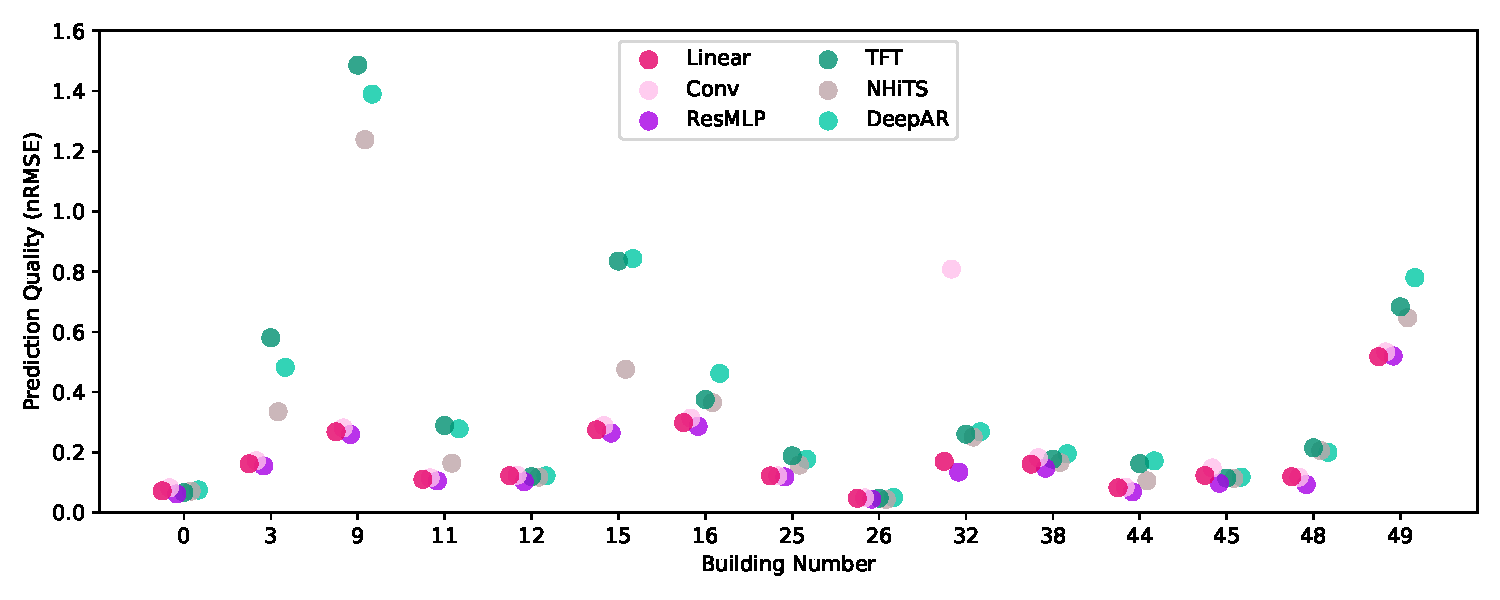
\includegraphics[width=0.9\linewidth]{Comparison/baseline_comparison_load_nRMSE.pdf}
    \label{fig:forecasting-baseline-load-comparison}
}
\bigskip

\subfloat[Correlation between model prediction accuracy and train-test data\\similarity metric value (lower Wasserstein metric means more similar data).]{
    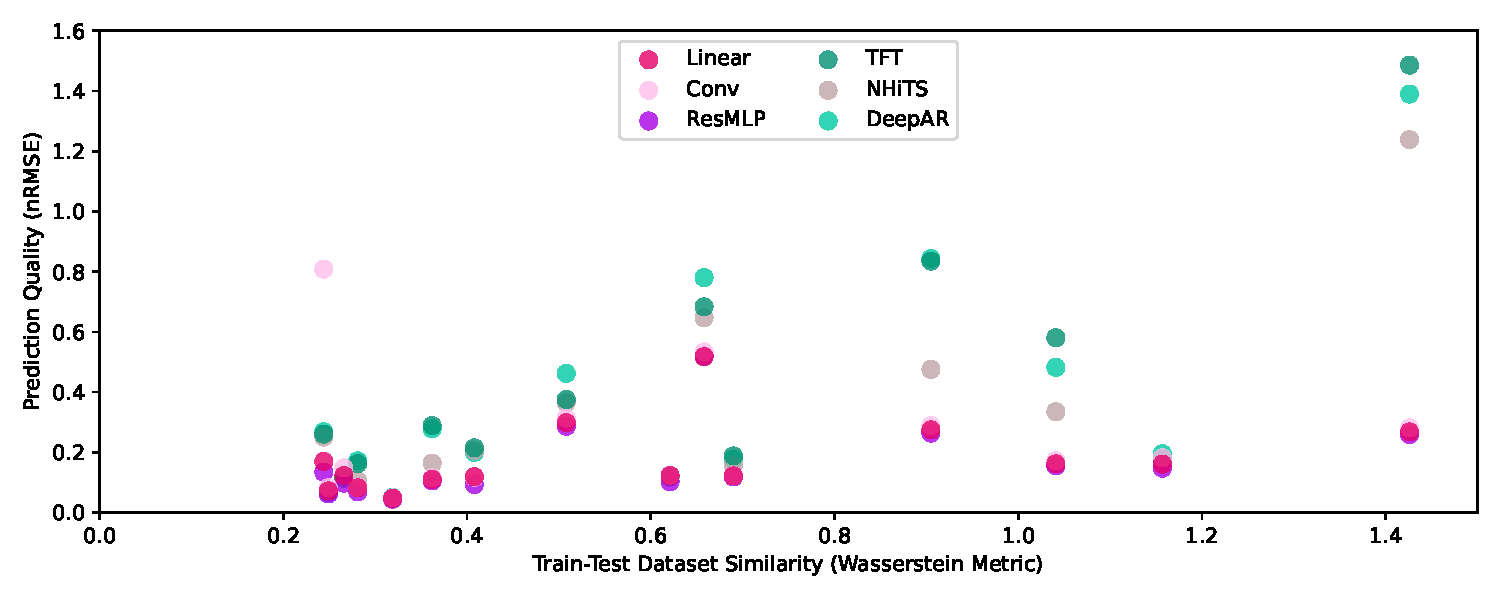
\includegraphics[width=0.9\linewidth]{Comparison/baseline_comparison_similarity_corr_nRMSE.pdf}
    \label{fig:forecasting-baseline-load-similarity-correlation}
}
\bigskip

\hspace*{\fill}
\subfloat[Pricing, carbon, solar prediction comparison.]{
    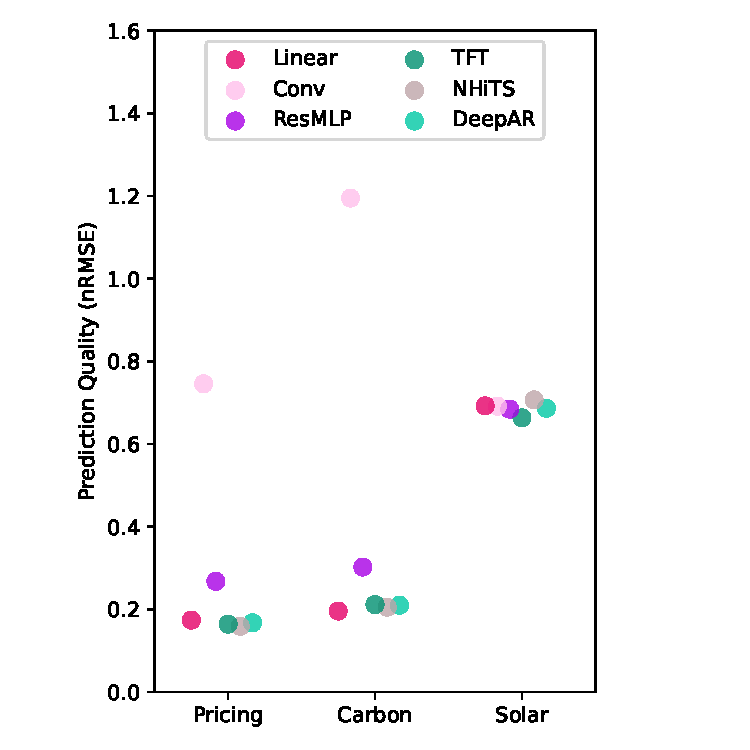
\includegraphics[height=6cm]{Comparison/baseline_comparison_PCS_nRMSE.pdf}
    \label{fig:forecasting-baseline-PCS-comparison}
}%
\hspace*{\fill}
\subfloat[Comparison of \glsxtrshort{mpc} operational performance using baseline forecasting models.]{
    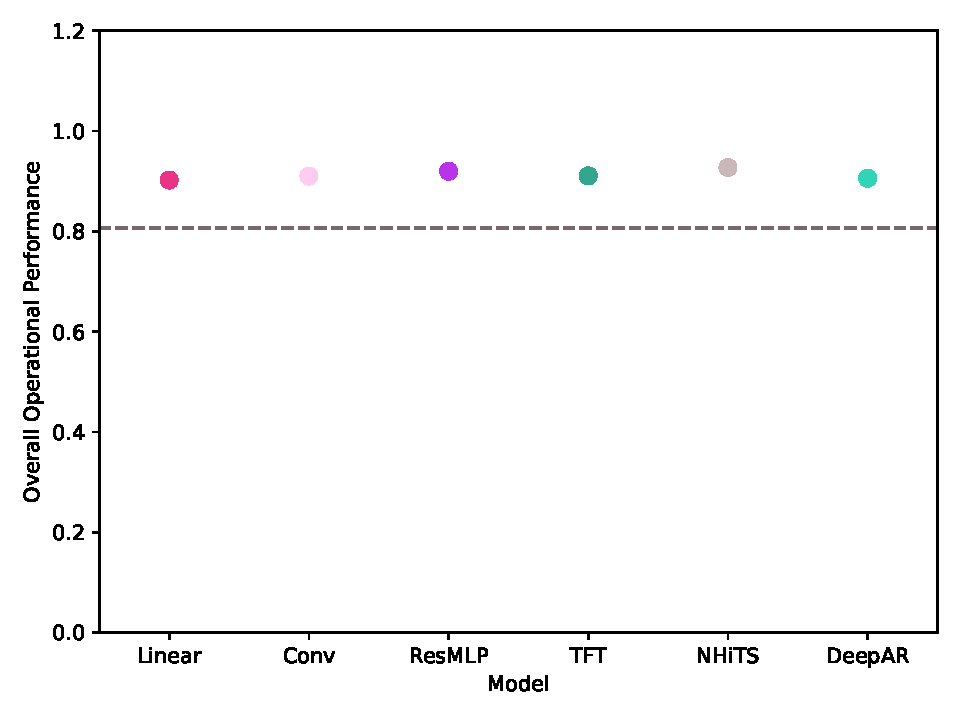
\includegraphics[height=6cm]{Comparison/baseline_comparison_evaluate.pdf}
    \label{fig:forecasting-baseline-evaluate-comparison}
}\hspace*{\fill}

\smallskip
\caption{Comparison of baseline prediction accuracy and operational performance of forecasting models.}
\label{fig:forecasting-baseline-comparison}
\end{figure}

These results indicate that simple neural models have sufficient expressivity to well capture the underlying trends in building energy usage, but learn sufficiently simple relationships about the data as to avoid the problem of over-fitting experienced by the complex models, leading to better generalisation in time. This suggests that the majority of the trends in the load data are present within the 1 week input window used by the simple models, which agrees with the strong daily and weekly trends of typical building energy usage, caused by building occupancy patterns. It is likely that annual trends are well captured by the mean value over the input window, as these trends are slow relative to the prediction length. Additionally, the predictions required by \glsxtrshort{mpc} are relatively short in length, 48 hours in this case, whereas the complex models are found to provide more stable predictions and greater overall accuracy for longer duration forecasts \citep{challu2023NHITSNeuralHierarchical,zhang2022TemporalFusionTransformer}.

Overall, simple neural models are able to provide analogous prediction accuracy to complex models across all prediction variables, and do so with substantially lower computational requirements. Table \ref{tab:forecasting-comp-times} provides the training time and inference time (time to generate forecasts) of the baseline models, and shows that simple models require roughly 500x less computation for inference. Hence, in practical systems the use of simple models would enable shorter prediction intervals, leading to higher frequency control, and allow for the use of lower cost compute hardware. Further, due to their high computational cost, the complex models were only able to use a 72 hour input window \citep{lopezsantos2022ApplicationTemporalFusion}. As a result, they have less information available to inform their predictions, likely limiting the accuracy they could achieve. Therefore, the computational efficiency of simple neural models enabling the use of longer input windows provides an additional advantage.\\

\begin{table}[h]
    \centering
    \renewcommand{\arraystretch}{1}
    \begin{tabularx}{\linewidth}{c|*{6}{X}} \toprule \toprule
        Model & Linear & Conv & ResMLP & TFT & NHiTS & DeepAR \\ \midrule
        Training time (hrs) & 12.3 & 26.8 & 13.4 & 8.9 & 15.2 & 9.3 \\
        Prediction inference time (s) & 29 & 73 & 146 & 15,222 & 15,289 & 74,991 \\ \bottomrule\bottomrule
    \end{tabularx}
    \smallskip
    \caption{Computation times for baseline models, trained on 8 years of data, and predicting for simulations of 2 years duration.}
    \label{tab:forecasting-comp-times}
\end{table}

The similar prediction accuracies of the tested models are found to lead to similar operational performance when used in the \glsxtrshort{mpc} scheme, see Fig. \ref{fig:forecasting-baseline-evaluate-comparison}, where the dashed line indicates the bound on operational performance achieved by an \glsxtrshort{mpc} scheme with perfect forecasts. The use of the \glsxtrshort{mpc} controllers with the specified battery systems leads to an average 8.7\% improvement in operational performance for the multi-building energy system, with a range of 7.3\% to 9.8\%.\\


\subsection{Model generalisation} \label{sec:forecasting-generalisation}

% Can data be reused? (Is it worth reusing?)
% Train on one building, test on another, how good is it?

When a solar-battery system using \glsxtrshort{mpc} is installed, high-resolution historic load metering data (e.g. from smart meters) may not be available for the building. In this case, the project must either be delayed to allow time for data collection, incurring a significant cost, or a prediction model trained on load data from another building must be used, potentially incurring an operational performance penalty due to worse prediction accuracy. Model reuse greatly reduces data collection requirements and the associated costs, however its appropriacy depends on the ability of load prediction models to generalise between buildings, and the trade-off between data cost savings and increased operational cost due to lower forecast accuracies.

The generalisation of prediction models between buildings is tested by using the baseline models trained on data from each of the 15 buildings to forecast electrical load for every other building. Fig. \ref{fig:forecasting-generalisation-violin} shows the distribution of relative forecast accuracies achieved by each model over all buildings (DeepAR is excluded due to excessive computational costs), where the y-axis plots the nRMSE forecast accuracy of the tested model (potentially trained on a different building) normalised by the forecast accuracy achieved by the model trained on data from the target building.\\

\begin{figure}[h]
    \centering
    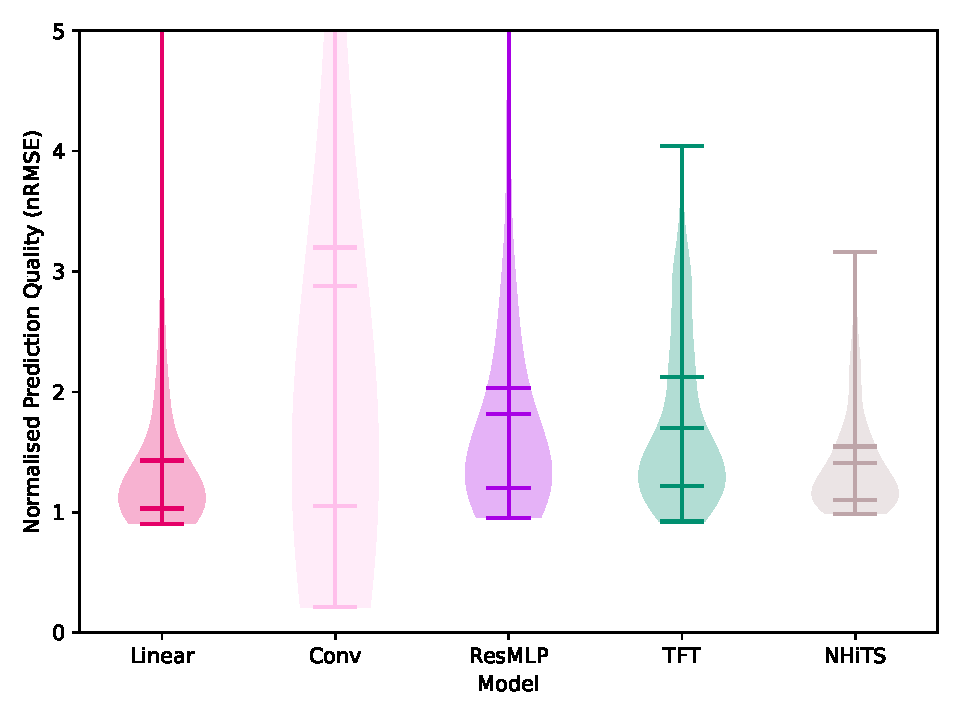
\includegraphics[width=0.7\linewidth]{Generalisation/generalisation_violin.pdf}
    \vspace*{-0.5cm}
    \caption{Comparison of forecasting model generalisation. Violin plot with quartiles indicated by horizontal lines.}
    \label{fig:forecasting-generalisation-violin}
\end{figure}
\bigskip

The Linear model provides similar generalisation performance to NHiTS, and is substantially better than all other models. It is proposed that the Linear model, being mechanistically equivalent to linear regression, achieves good generalisation as it learns relatively simple relationships about the load data, which are consistent between buildings. Whereas NHiTS achieves good generalisation due to its behaviour of generating smooth forecasts \citep{challu2023NHITSNeuralHierarchical}, making it less susceptible to producing erratic and inaccurate predictions with unseen input data. As before, TFT suffers from over-fitting, leading to relatively poor generalisation. Whilst the Conv model was able to provide good generalisation in time where the dataset similarity was close, indicated by small Wasserstein metric values in Fig. \ref{fig:forecasting-baseline-load-similarity-correlation}, between buildings the load data is much less similar, and the relationships learned by the Conv model are no longer valid, leading to poor prediction accuracy. It is suggested this is due to the features learned by the pooling process no longer being pertinent for the new building.\\

If a pre-trained Linear model is selected for reuse at random, the average prediction accuracy is substantially worse than a model trained on data collected from the target building (45\% higher nRMSE, corresponding to the mean of the violin plot). However, in a real scenario where an ensemble of pre-trained models is available, the smart energy storage system designer could reuse a model from a building that is expected to be similar to the target building (e.g. by size, usage type, envelope characteristics, load dynamics, etc.), to maximise the likelihood of good generalisation. A load profile similarity metric is additionally proposed as a way off assessing the similarity of building load dynamics for the purposes of model reuse. This similarity metric is based on the similarity of the distributions of underlying mode shapes within each load profile, and is referred to as the `Wasserstein similarity metric' as it uses the Wasserstein distance between mode shape coefficient distributions. Appendix \ref{app:forecasting-similarity-metric} describes the calculation of similarity metric values. The correlation between generalisation of the Linear model and the Wasserstein similarity metric values between the training datasets of the reused model building and target building is shown in Fig. \ref{fig:forecasting-generalisation-linear-Wass-corr}. The cluster of points in the bottom left indicates that buildings with similar load profiles (low Wasserstein metric values) can provide models that achieve good generalisation. When selecting models for reuse by minimising the Wasserstein metric, the average relative prediction accuracy improves to an 11\% increase in nRMSE, with a range of -7.9\% to +52.6\%, showing that some reused models outperform those trained on the true building training dataset.

\begin{figure}[h]
    \centering
    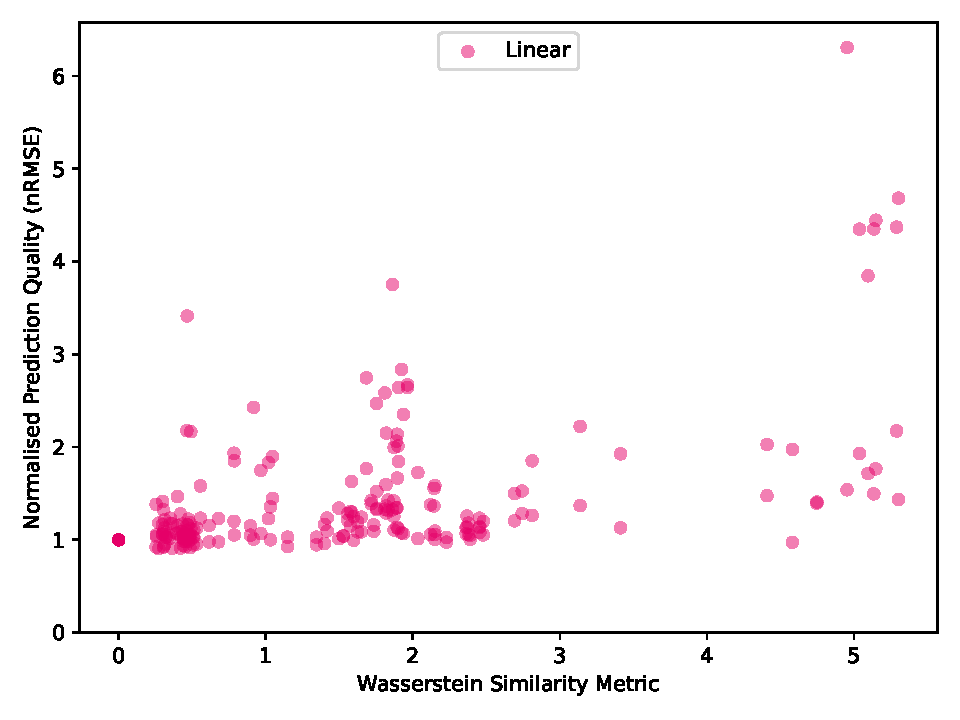
\includegraphics[width=0.7\linewidth]{Generalisation/generalisation_linear_similarity_corr.pdf}
    \caption{Correlation between Linear model generalisation and training dataset similarity metric values.}
    \label{fig:forecasting-generalisation-linear-Wass-corr}
\end{figure}

These results show that when developing a load forecasting model for a new building system where little or no data is available, the reuse of forecasting models trained on existing buildings provides a promising\footnote{Further work is required to determine the feasibility of identifying similar buildings from the model ensemble in practice. Whilst a small sample of load data from the target building could be used to approximate the Wasserstein similarity metric, the quality of this approximation must be weighed against the forecast accuracy that could be achieved by a model trained using that data. Though, additional information on the building, such as usage type, could be used to guide model selection for reuse.} alternative to the collection of data and training of a building specific model, and the associated costs. However, reusing prediction models increases uncertainty in the operational performance the \glsxtrshort{mpc} system will achieve, as models trained on load data from buildings similar to the target building do not always provide good prediction accuracy, as shown by the wide range of reused model accuracies.


\newpage
\subsection{Data efficiency} \label{sec:forecasting-data-efficiency}

% Can the data efficiency of models be improved? What are the trade-offs between data usage and prediction quality?

Data required for developing forecasting models incurs cost from both its acquisition and the computation required to exploit it. However, using longer durations of training data or additional data variables can increase forecast accuracy, resulting in lower operational cost of the energy system. Therefore, any measures to reduce the quantity of data used must be traded-off against the corresponding decrease in prediction accuracy. This section explores a series of aspects of data efficiency and their effect on forecast accuracy. Subsequently, Section \ref{sec:forecasting-control-sensitivity} investigates the impact of forecast accuracy on operational performance of the \glsxtrshort{mpc}.

Testing data efficiency requires several versions of a prediction model to be trained. Due to computational limitations, for some data efficiency tests only the Linear prediction model is studied, as the complex models are too computationally expensive, and results from previous sections show the Linear model is the best performing simple model.

\subsubsection{Volume of training data} \label{sec:forecasting-data-efficiency-training-data}

% Use less data, what happens to prediction quality?

Using greater volumes of training data, longer durations of historic measurements of buildings, can improve model prediction accuracy by avoiding over-fitting, improving temporal generalisability, but comes at a roughly linear cost. The trade-off between the length of training data used, the combined duration of the train and validate datasets, and forecast accuracy is investigated by training prediction models on subsets of the building energy dataset of varying durations from 8 years, the maximum duration available, to 3 months (one season), the shortest duration tested in \citep{choi2023PerformanceEvaluationDeep}. For the complex models, at least 2 years of training data was required due to the use of temporal covariates. Fig. \ref{fig:forecasting-data-eff-n-training-years} plots the proportional improvement in prediction accuracy of each model (negative improvement shows worsening model accuracy) compared to baseline when training using different data volumes. Across a broad range of model architectures, reducing training data length down to 2 years has a limited impact on prediction accuracy, in some cases improving prediction accuracy. Trends differ between prediction variables, however for the Linear model, in the majority of cases there is a small prediction accuracy penalty between 8 and 1 years of training data, and then a rapid worsening of forecasting accuracy below 6 months.
This indicates that when making data collection decisions to support prediction model development for building electrical energy systems, at most 2 years of measurement data should be gathered. However, at least two seasons of data (6 months) are required to prevent model over-fitting and learn trends which generalise across seasons.

\begin{figure}
    \centering
    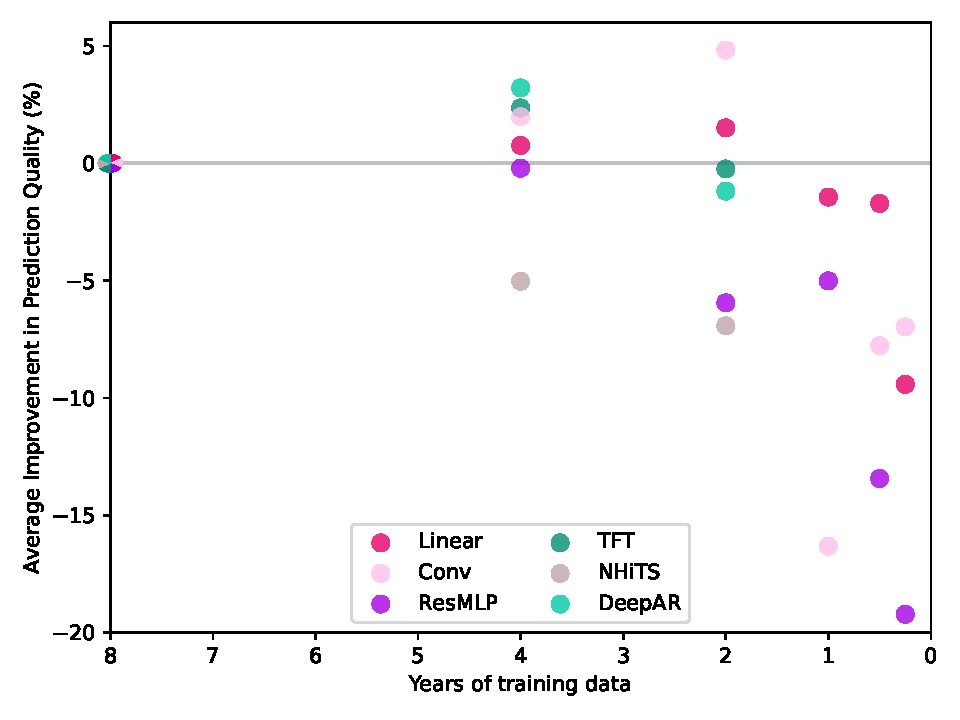
\includegraphics[width=0.7\linewidth]{Data_Efficiency/prediction_vs_n_training_years.pdf}
    \caption{Average improvement in prediction accuracy over all prediction variables with years of data used for training.}
    \label{fig:forecasting-data-eff-n-training-years}
\end{figure}


\paragraph{Screening training data using change-points} \label{sec:forecasting-data-efficiency-change-point}

% Use less data, excluding training data in an intelligent way, what happens to prediction quality?
% Use identified change-points from analysis in Section \ref{sec:change-points} to see if removal of non-representative training data can improve model performance and data efficiency - use multiple change-points only.
% Do our results correspond with those from \citep{choi2023PerformanceEvaluationDeep} that not all additional training data is useful, only the similar sections? Acknowledge data similarity study in Wonjun's paper in discussion - yes, but trade-off between use of non-representative data and having enough data to avoid over-fitting. Unlike Wonjun's results, we are testing on 2years of data (he only tests on 0.1yrs), so I think we need at least a full years of data to capture all of the seasonality in the model.
% Note this is a very simple screening method, and assessing similarity of chunks to validation data would like provide a better method (though this assumes validation data is most representative of test data...), we could use the Wasserstein metric for this.

Once building data has been gathered, there remains a question as to whether all of the available data should be used for training, or whether some data should be excluded to improve model prediction. For instance, if data that is non-representative of the present building load dynamics can be excluded, prediction accuracy can be improved alongside data efficiency.
Change-point analysis can be used to screen training data for this purpose, by detecting changes in building load dynamics and excluding data preceding the change from training. A change-point analysis using the BEAST algorithm \citep{zhao2019DetectingChangepointTrend} was performed on the building load dataset, described in Appendix \ref{app:forecasting-change-points}. Points where changes in load trend were detected were used to screen the training data for 7 selected buildings. In order to allow a better analysis of the detected change-points, the training dataset was increased to 7 years (2010-2016), leaving 1 year of validation data (2017). Linear prediction models were trained using sections of the training data starting at each detected change-point and running to the end of 2016.

\begin{figure}
    \centering
    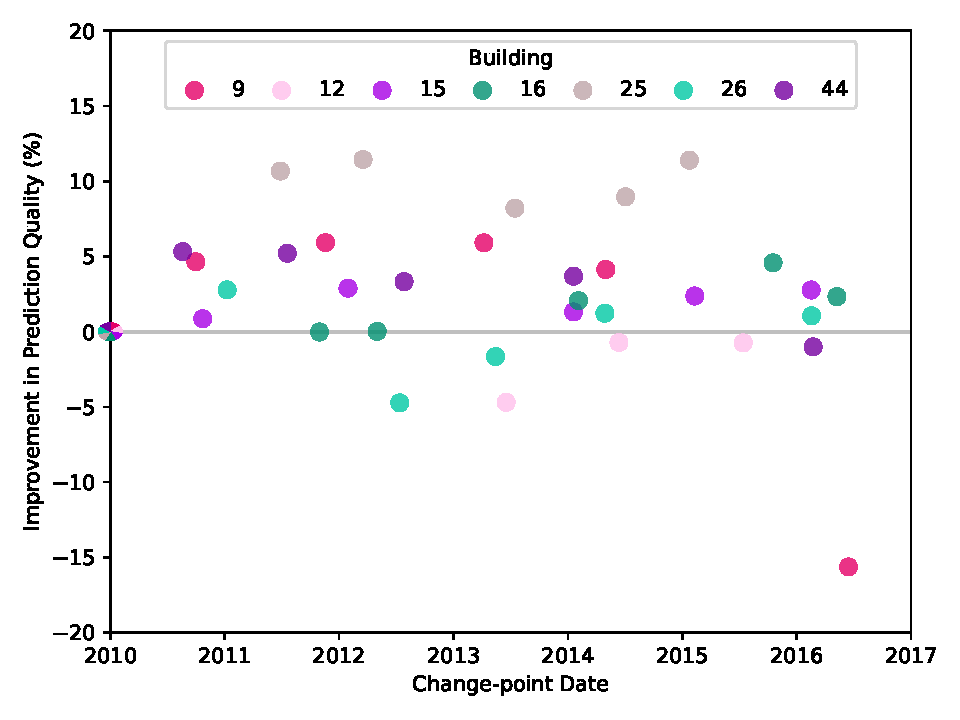
\includegraphics[width=0.7\linewidth]{Data_Efficiency/chagepoint_prediction_performance.pdf}
    \caption{Improvement in prediction accuracy of models trained using data from change-points onward.}
    \label{fig:forecasting-data-eff-changepoints}
\end{figure}

Fig. \ref{fig:forecasting-data-eff-changepoints} shows the relative improvements in prediction accuracy of models trained on data screened using change-points, compared to the case where the full 7 years of available data is used, where the x-axis position indicates the timing of the change-point. For most buildings, screening the training data using change-points improves prediction accuracy, indicating that non-representative data is being removed from the training dataset. This suggests that ex-post training data screening can be used to improve model accuracy whilst reducing the quantity of training data used, and so computational cost. These results correspond with the findings of \citep{choi2023PerformanceEvaluationDeep}, which shows that additional training data only improves prediction accuracy if it is sufficiently similar to the test data, and can reduce accuracy when insufficiently similar. However, the results of this study demonstrate an additional consideration, which is that prediction accuracy worsens substantially when insufficient training data volume is used. This suggests a trade-off between having enough data to avoid over-fitting, and removing non-representative data which causes over-generalisation of the model. Figures \ref{fig:forecasting-data-eff-n-training-years} \& \ref{fig:forecasting-data-eff-changepoints} indicate that at least 1 year of training data is required to achieve good prediction accuracy, after which only sufficiently similar data should be included in the training dataset. The reason for the difference in results compared to \citep{choi2023PerformanceEvaluationDeep} is likely due to this study testing model prediction accuracy on 2 years of data, compared to 0.1 years in \citep{choi2023PerformanceEvaluationDeep}. As a result, models in this study must capture the seasonality of building load dynamics, hence requiring at least 1 year of training data to achieve good prediction accuracy.

The data screening method considered in this study is relatively simple, using change-points to exclude data by classifying it as `non-representative' of current behaviour. More advance techniques could be created by quantifying the similarity between the sections of data identified using the change-points and the validation data, e.g. using the Wasserstein similarity metric, and selecting sections of data to use in the training dataset using both the probability of a true change having occurred and the data similarity metrics.

Change-point analysis can also be used online to detect real time changes in building load dynamics and provide indication of when the prediction models should be updated (i.e. retrained using recent data), due to the training data of the current model no longer being representative of the building behaviour, causing reduced prediction accuracy. This is particularly pertinent in the context of climate change, which is expected to significantly impact the energy usage behaviour of buildings, for instance reducing peak heating loads due to higher winter temperatures, and increasing summer electrical loads to provide cooling during prolonged heat waves.

\subsubsection{Data features} \label{sec:forecasting-data-efficiency-data-features}

% Use less data by not measuring some stuff, what happens to prediction quality?

The variables that can be monitored in building energy systems are often well correlated, for example ambient temperature and electrical load. As a result, covariates can be used by prediction models to attempt to identify underlying links between the variables and improve forecast accuracy. However, the use of additional data variables (features) incurs a cost from both the collection and exploitation of the extra data, for instance the purchase of proprietary weather forecasts. The impact of feature selection on forecast accuracy is investigated by comparing the prediction accuracy of models trained using varying numbers of data features. The Pearson correlation coefficient between the 11 data features available in the building energy dataset are shown for the case of Building 0 in Fig. \ref{fig:forecasting-data-eff-variable-correlations}. Linear prediction models were trained using the $n$ most correlated variables/features for each of the electrical load, solar generation, electricity price, and carbon intensity target variables. Feature selection was performed separately for each case by ranking Pearson correlation coefficients between the target variable and all other available covariates. Fig. \ref{fig:forecasting-data-eff-n-variables} shows the impact of the number of data features used by the models on forecast accuracy. For most prediction variables, the inclusion of additional data features worsens forecast accuracy. Several factors could contribute to this behaviour:
\begin{itemize}
    %\setlength\itemsep{0ex}
    \item Over-fitting \citep{hawkins2004ProblemOverfitting} : The incorporation of an excessive number of features may lead the model to over-fit the training data, worsening its predictions for unseen data.
    \item Multi-collinearity \citep{farrar1967MulticollinearityRegressionAnalysis} : The presence of highly correlated features can destabilize the model, resulting in worse prediction accuracy.
    \item Curse of Dimensionality \citep{verleysen2005CurseDimensionalityData} : An increase in the number of features increases the dimensionality of the data, which can lead to data sparsity and degradation of prediction accuracy.
\end{itemize}

\begin{figure}
    \centering
    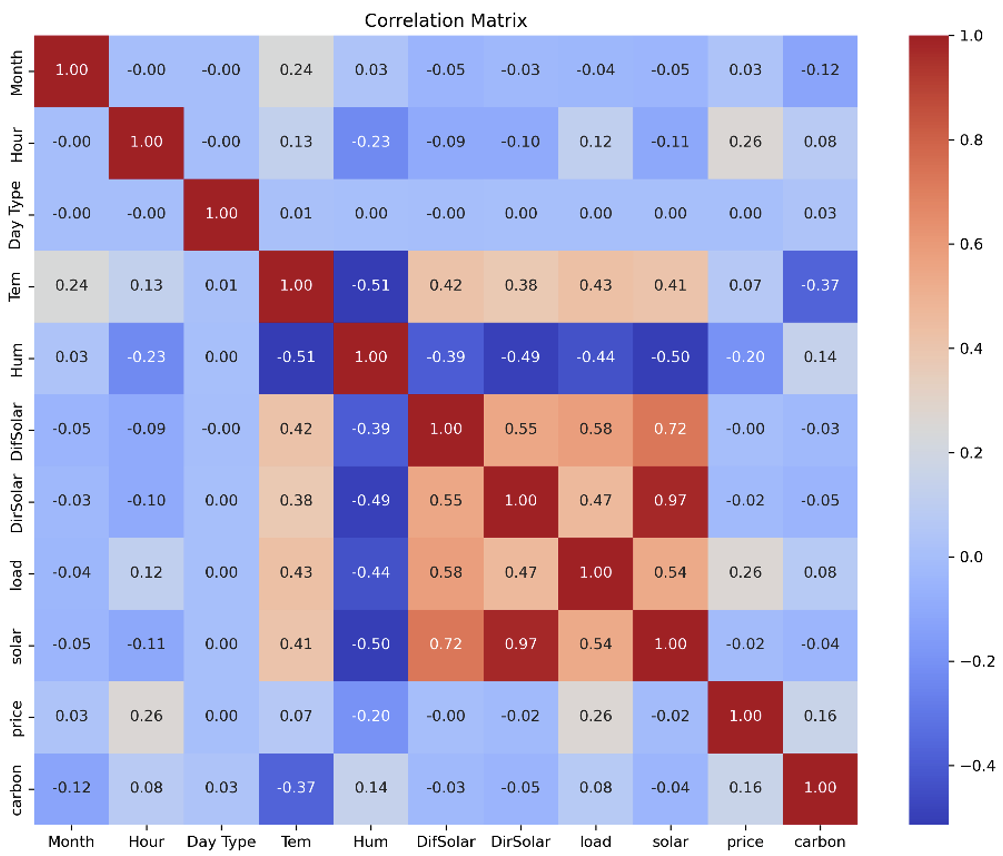
\includegraphics[width=0.5\linewidth]{Data_Efficiency/variable_correleations.png}
    \caption{Pearson correlation between data variables for Building 0.}
    \label{fig:forecasting-data-eff-variable-correlations}
\end{figure}

\begin{figure}[h]
    \centering
    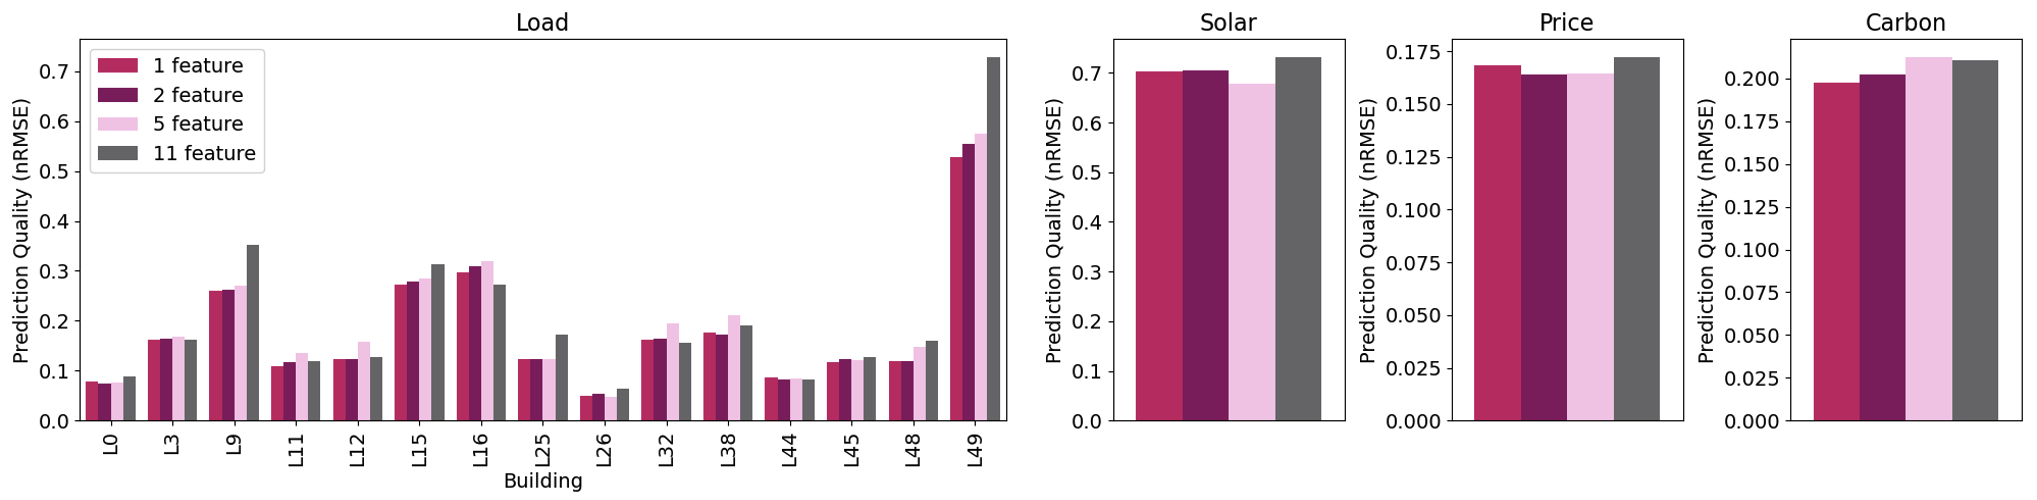
\includegraphics[width=\linewidth]{Data_Efficiency/prediction_vs_n_variables.png}
    \caption{Variation of prediction accuracy with no. of data features included in Linear model.}
    \label{fig:forecasting-data-eff-n-variables}
\end{figure}

These results show that testing should be performed before decisions are made regarding the collection of covariate data to ensure that, for the type of system in question, its use will firstly improve prediction accuracy, and secondly that said accuracy improvements warrant the cost of the data. This study considers a simple, correlation based feature selection method, however more advanced, optimization based techniques \citep{gonzalez-vidal2019MethodologyEnergyMultivariate,kim2020ElectricityLoadForecasting} could be used to determine the set of available features which provides the optimal trade-off between data cost and model prediction accuracy.

\subsubsection{Online training} \label{sec:forecasting-online-training}

% Use all of the data you have available from realtime measurements, how can prediction quality be improved? And is it worth the extra hardware and complexity of the deployed system?

During building operation monitoring systems continuously collect operational data. The characteristics of building behaviour can change during operation due to external factors such as weather \& climate, occupancy, and equipment degradation \& maintenance. Continuous online training updates the predictive models using the collected monitoring data, improving the model's ability to adapt to dynamic changes in building behaviour. A version of the Linear prediction model with online training is implemented to investigate the impact of online training frequency on model accuracy. The model is updated online by tuning the model parameters (retraining) using a sliding window of training data with length equal to the update frequency.
The prediction accuracy of models updated at different frequencies is plotted in Fig. \ref{fig:forecasting-data-eff-update-freq}. Higher update frequencies led to increased prediction accuracy across all prediction variables. For example, prediction accuracy for grid electricity price improved by 15.7\%, 14.0\%, 12.1\%, and 8.1\% when updated monthly, quarterly, semi-annually, and annually, respectively, compared to the baseline model which is not trained online. Online training allows the prediction model to adapt to changes in the underlying trends which occur over time, as it can learn the trends in recent data. This improves prediction accuracy as the model does not need to generalise in time, as it is trained (updated) on data that is representative of the current prediction horizon.
Therefore, it is expected that the additional computational hardware and system complexity required for online trained prediction models will be worthwhile in practical systems.

\begin{figure}[h]
    \centering
    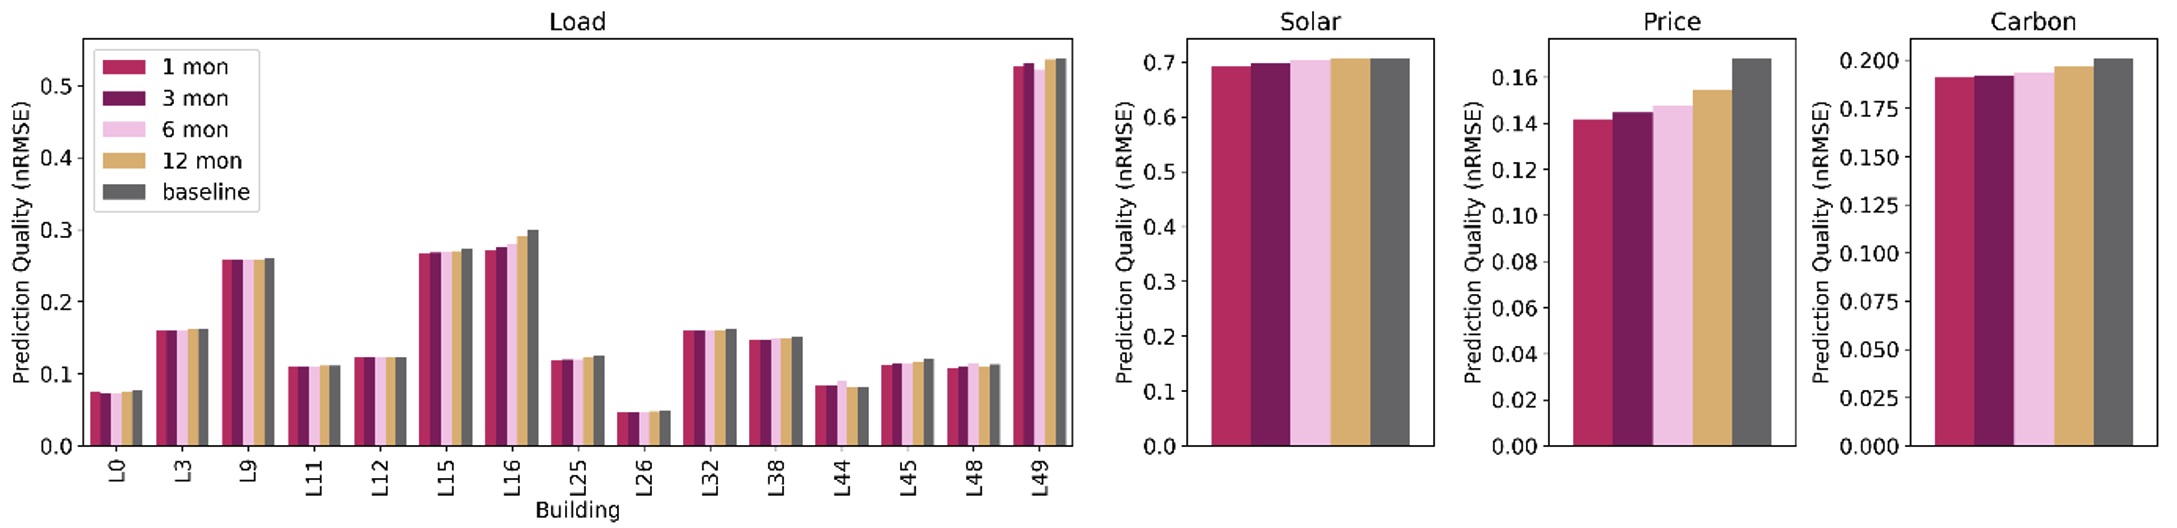
\includegraphics[width=\linewidth]{Data_Efficiency/prediction_vs_update_freq.png}
    \caption{Variation of prediction accuracy with online update frequency.}
    \label{fig:forecasting-data-eff-update-freq}
\end{figure}


\newpage
\subsection{Sensitivity of Model Predictive Control to forecast accuracy} \label{sec:forecasting-control-sensitivity}

% Tie forecasting analysis in with the simulation framework and explain how this provides a methodology for determining whether investment in additional data is economic -- e.g. model reuse vs direct data collection, data efficiency measures above, or purchase of external forecasts from service.
% May require some discussion about realism of noise model and correlation between results obtained and performance of true prediction models (grid performance poor for this synthetic noisy model which distorts results). But regardless this analysis provides an indicative method for how this type of economic analysis of optimal data requirements would be done. Opportunity for significant further work - create noise model calibrated to performance-accuracy trade-off of practical prediction models, which hopefully provides a better representation of the underlying inaccuracy patterns.

Whether investments in additional data to improve forecast accuracy provide net benefit to the operation of a smart energy storage system depends on the resulting improvements in operational performance achieved by the \glsxtrshort{mpc} controller. The determination of optimal data collection strategies therefore requires quantification of the relationship between forecast accuracy and \glsxtrshort{mpc} operational performance. To investigate this in a controlled setting, the operational performance achieved by the tested \glsxtrshort{mpc} scheme is evaluated with the use of synthetic forecasts. The synthetic forecasts are produced by adding a Gaussian random walk noise component to the ground-truth values, as described in Eq. \ref{eq:forecasting-GRWN},

\begin{equation} \label{eq:forecasting-GRWN}
    f_{\mathsmaller{\textrm{GRW}}}^v[t,\tau] = v_{t+\tau} + \sum_{j=1}^{\tau} w_j^{\sigma} \qquad \textrm{s.t.} \:\: w_j^{\sigma} \:\: \textrm{i.i.d.} \:\: \mathcal{N}\!\left( \mu{=}0, \sigma^2 \right)
\end{equation}

where $v_{t+\tau}$ is the ground-truth value of variable $v$ at instance $\tau$ in the planning horizon of the forecast created at time $t$, and the noise level $\sigma$ can be selected.

The \glsxtrshort{mpc} scheme using these synthetic forecasts for all prediction variables is tested at varying noise levels. Fig. \ref{fig:forecasting-control-sens-obj-vs-noise} shows the resulting operational performance of \glsxtrshort{mpc}, as well as the three components it is comprised of (electricity price, carbon emissions, and grid impact), as the prediction accuracy of the synthetic forecasts varies. Fig. \ref{fig:forecasting-control-sens-control-vs-noise-type} shows the variation in overall operational performance of the \glsxtrshort{mpc} when synthetic forecasts are used for each type of prediction variable in turn, with perfect forecasts used for all other variables. The horizontal line at 1 indicates the performance of the building energy system without battery control, which is the point at which the \glsxtrshort{mpc} controller becomes redundant.

The results show that the tested \glsxtrshort{mpc} scheme is most sensitive to the forecast accuracy of the grid electricity price and carbon intensity variables, suggesting that the most resource and expense should be invested in producing accurate forecasts of the grid conditions. Additionally, whilst the prediction models tested in this study performed worst when forecasting solar generation, see Fig. \ref{fig:forecasting-baseline-PCS-comparison}, it may not be worth expending additional resource to improve these forecasts as the \glsxtrshort{mpc} scheme is least sensitive to this variable. Though the grid component of operational performance is found to be by far the most sensitive to forecast accuracy, this is likely due to the synthetic forecast model used\footnote{In the synthetic forecast model used, the Gaussian random walk noise component is regenerated at each time instance. This leads to the generation of forecasts which are correct on average, but can cause the \glsxtrshort{mpc} controller to take opposing energy management strategies in successive time steps, leading to large magnitudes of energy flows from the battery to correct the strategy. Further work is required to create a noise model for synthetic forecasts that is calibrated to the operational performance vs forecast accuracy trade-off of practical prediction models. With such a noise model, the experimental method demonstrated could be used to quantify the economic advantage of forecast accuracy improvements to support decision making regarding data collection.} for the development of forecasting models in practical smart energy storage systems, and is not considered to be reflective of the behaviour of real prediction models.

\begin{figure}[p]
    \centering

    \subfloat[Variation of operational performance components with amplitude of noise on all prediction variables.]{
        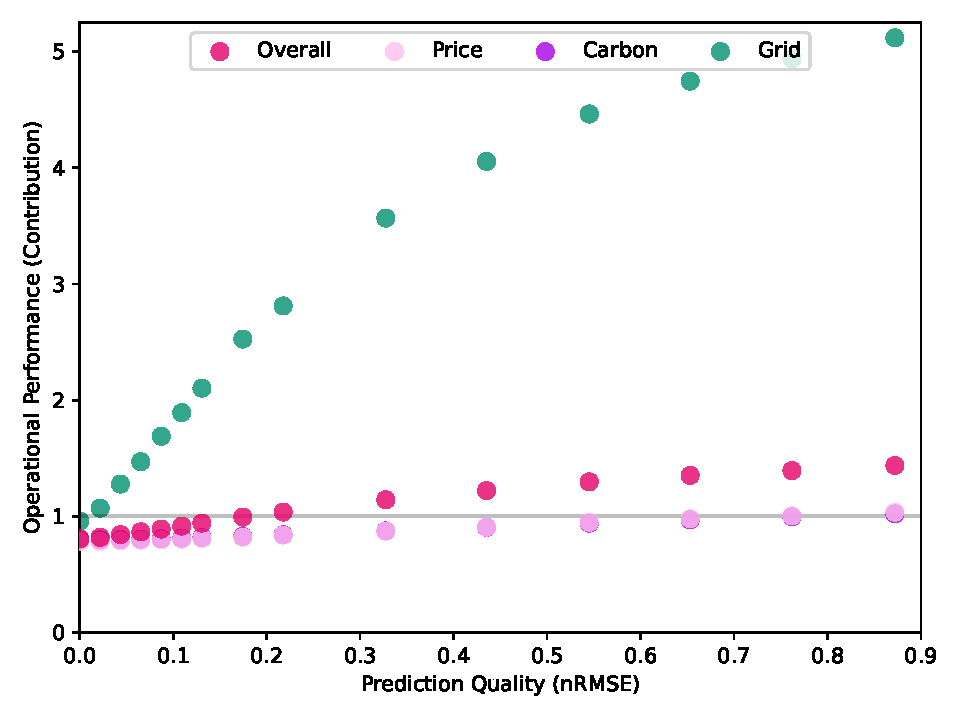
\includegraphics[width=0.7\linewidth]{Control_Sensitivity/control_obj_vs_noise.pdf}
        \label{fig:forecasting-control-sens-obj-vs-noise}
    }
    \bigskip

    \subfloat[Variation of overall operational performance with amplitude of noise on each type of prediction variable.]{
        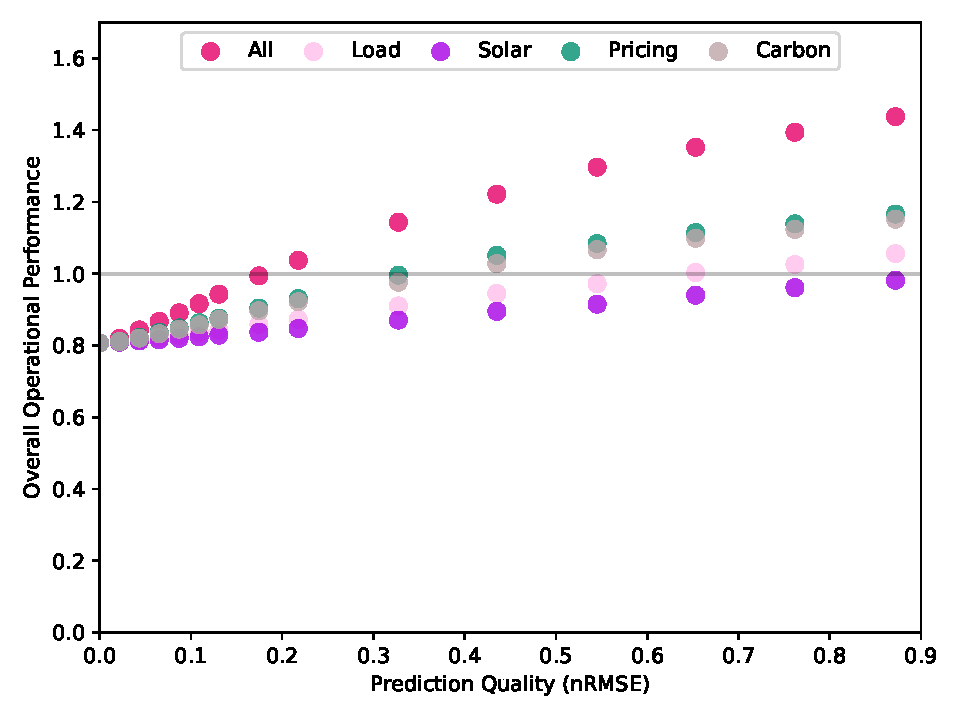
\includegraphics[width=0.7\linewidth]{Control_Sensitivity/control_performance_vs_noise_type.pdf}
        \label{fig:forecasting-control-sens-control-vs-noise-type}
    }
    \smallskip
    \caption{Sensitivity of operational performance to synthetic forecast noise simulating prediction inaccuracy.} \label{fig:forecasting-control-sens}
\end{figure}


\newpage
%********************************** Conclusions **************************************
\section{Conclusions} \label{sec:forecasting-conclusions}

This chapter investigated the impacts of data on the accuracy of machine learning based forecasting models for building operational conditions, and the resulting operational performance of a \glsxtrlong{mpc} (\glsxtrshort{mpc}) scheme in a multi-building energy system with distributed generation and storage. Experiments were conducted using a large-scale dataset of electrical load measurements from buildings in the Cambridge University Estates.

A simple linear multi-layer perceptron model (Linear) using DMS prediction was found to achieve equivalent forecast accuracy to high-complexity, state-of-the-art machine learning models in a setting without data limitations, but has substantial advantages regarding data efficiency and generalisation performance. So, this simple neural model is better suited for use in practical \glsxtrshort{mpc} systems due to its lower data and computational requirements, and better performance on new load dynamics.

Using more than 2 years of hourly resolved training data did not provide significant improvements in prediction accuracy for most of the models tested, indicating that the collection of monitoring data for longer durations is unnecessary for the development of performant \glsxtrshort{mpc} schemes. Further, screening training data using change-point analysis to remove low similarity data was able to simultaneously improve data efficiency and prediction accuracy, provided at least 1 year of training data was kept. This could also be achieved through the removal of redundant data features from models.

The reuse of Linear models for load prediction between buildings was shown to be an effective way of reducing data collection requirements. When selecting models for reuse using a proposed load profile similarity metric based on the Wasserstein distance between fPCA coefficient distributions, model reuse led to an average 11\% increase in prediction error. However in comparison, models trained using only 3 months of building specific data provided forecasts with an average 9.9\% increase in error compared to the baseline. Additionally, online training of prediction models was shown to be highly beneficial, with higher update frequencies providing greater forecast accuracy improvements, of up to 15.7\% for the case of monthly updating. Hence, monitoring data should be used to update reused prediction models in situ to tailor them to the building system, ultimately replacing the reused model. The results suggest that, by exploiting existing building energy datasets to pre-train models, in many cases sufficient forecast accuracy can be achieved without the collection of any building load data prior to the installation of the system.

The relationship between forecast accuracy and operational performance of the \glsxtrshort{mpc} controller was investigated for synthetic forecasts, which showed the \glsxtrshort{mpc} scheme is most sensitive to grid electricity price and carbon intensity prediction accuracy. This indicates that the most effort and expense should be spent on developing or purchasing high accuracy forecasts of the grid conditions, as these will provide the greatest improvement in operational performance of the controller.

% In some sense you can think of gathering more data as reducing uncertainty in the building behaviour, but it's very difficult to come up with a statistical model of this, so VoI isn't super appropriate - in fact from what we've seen, more data doesn't always lead to improvements in performance. We need to be a little bit more anecdotal, as this is a pretty complex data setting
% Comparison of general/foundation models vs building specific models is explored in the project with Fabian

In this chapter, the operational performance of the \glsxtrshort{mpc} controller was studied using a relative performance metric\footnote{This was done to match the goal of the CityLearn Challenge 2023 \citep{nagy2023CityLearnChallenge2023}.}. However, the analysis could be repeated using an economic performance metric. This would allow the financial benefit of data for improving forecast accuracy to be quantified. By comparing to the costs of data collection, building operators could determine whether expenditure on additional data collection or commercial forecasts is beneficial, i.e. whether the costs of data are outweighed by the improvements in operational performance provided. And if so, the results could also be used to determine the optimal data collection strategy.

This analysis would be conceptually quite similar to a \glsxtrlong{voi} analysis, and has the same objective. However in this case using the \glsxtrshort{voi} methodology is not appropriate. While collecting more training data could be viewed as reducing uncertainty in the behaviour of a building, it is not clear how a statistical model of this uncertainty could be constructed, and whether the setup is really compatible with a statistical viewpoint\footnote{Data collected other buildings could be viewed as a prior distribution for the load data of the target building. This is the modelling approach taken in \Cref{chap:districts}. A prediction model trained on this data, often referred to as a general or foundation model, could be seen as a prior decision. This general model could then be updated using data collected from the target building in a Bayesian-like fashion, improving prediction accuracy for the target building. An approach similar to this is taken in \citep{raisch2025AdaptingChangeComparison} to study the impact of data on the accuracy of system dynamics models.}.
The analysis in \Cref{sec:forecasting-data-efficiency} showed that collecting more data does not always improve prediction accuracy, as building load dynamics can change over time, and additional historic data is not always representative of the current behaviour, meaning it can worsen model training. This breaks one of the key assumptions of the \glsxtrshort{voi} methodology. An analysis using synthetic data could be performed, however it would be difficult to justify or validate its applicability to real-world energy systems.
So due to the complexity of the data required to study forecasting accuracy, the case study based approach used in this chapter is better suited for investigating data collection requirements for forecasting.


\newpage
%********************************** Chapter appendices  **************************************
\begin{subappendices}
    \section{Multi-building energy system asset specification} \label{app:forecasting-system-spec}

    The specifications of the distributed generation and storage assets for the multi-building energy system simulated in this study are provided in Table \ref{tab:forecasting-energy-assets}. The battery power capacities are set to be 3 times the mean building electrical load in the test dataset, the battery energy capacities are set to be able to provide 24 hours of that mean electrical load, and the solar PV power capacities are set by assuming 90\% of the roof area of each building is filled by solar panels of power density 0.15 kWp/m$^2$.\\

    \begin{table}[h]
        \centering
        \renewcommand{\arraystretch}{1}
        \begin{tabularx}{\linewidth}{c|*{4}{>{\setlength{\baselineskip}{.5\baselineskip}}Y}} \toprule \toprule
            Building & Battery power capacity (kW) & Battery energy capacity (kW) & Battery efficiency (\%) & Solar PV power capacity (kWp) \\ \midrule
            0 & 531 & 4246 & 90 & 461 \\
            3 & 60 & 478 & 90 & 38 \\
            9 & 14 & 108 & 90 & 20 \\
            11 & 342 & 2736 & 90 & 41 \\
            12 & 98 & 780 & 90 & 89 \\
            15 & 203 & 1622 & 90 & 143 \\
            16 & 306 & 2448 & 90 & 120 \\
            25 & 275 & 2198 & 90 & 118 \\
            26 & 1001 & 8006 & 90 & 136 \\
            32 & 157 & 1255 & 90 & 166 \\
            38 & 58 & 461 & 90 & 46 \\
            44 & 1084 & 8674 & 90 & 663 \\
            45 & 1245 & 9962 & 90 & 437 \\
            48 & 622 & 4973 & 90 & 500 \\
            49 & 57 & 458 & 90 & 258 \\
            \bottomrule\bottomrule
        \end{tabularx}
        \smallskip
        \caption{Specification of distributed energy assets in simulated multi-building energy system.}
        \label{tab:forecasting-energy-assets}
    \end{table}


    \newpage
    \section{\glsxtrshort{mpc} planning horizon} \label{app:forecasting-tau}

    % Provide references and plot to justify use of $\tau=48$ - good trade-off of near-optimal control performance and feasible computation time (+ no failures)

    The planning horizon used in a \glsxtrshort{mpc} scheme determines its ability to effectively arbitrage energy and meet the operational objectives of energy management. Previous studies show that a planning horizon of 24 hours is sufficient when controlling HVAC systems \citep{oldewurtel2012UseModelPredictive}, and recommend 48 hours as a suitable value for systems with distributed solar and storage \citep{thieblemont2017PredictiveControlStrategies}.

    To demonstrate the suitability of a planning horizon of $T=48$hrs for the experiments on the test system in this study, the operational performance of the \glsxtrshort{mpc} scheme using perfect forecasts is evaluated over varying planning horizon lengths, along with the computational time required to solve the Linear Programs for the simulations, shown in Fig. \ref{fig:forecasting-planning-horizon}. It can be seen that $T=48$hrs provides near-optimal control performance at a reasonable computation time, and so is a suitable choice for the experiments.\\

    \begin{figure}[h]
        \centering
        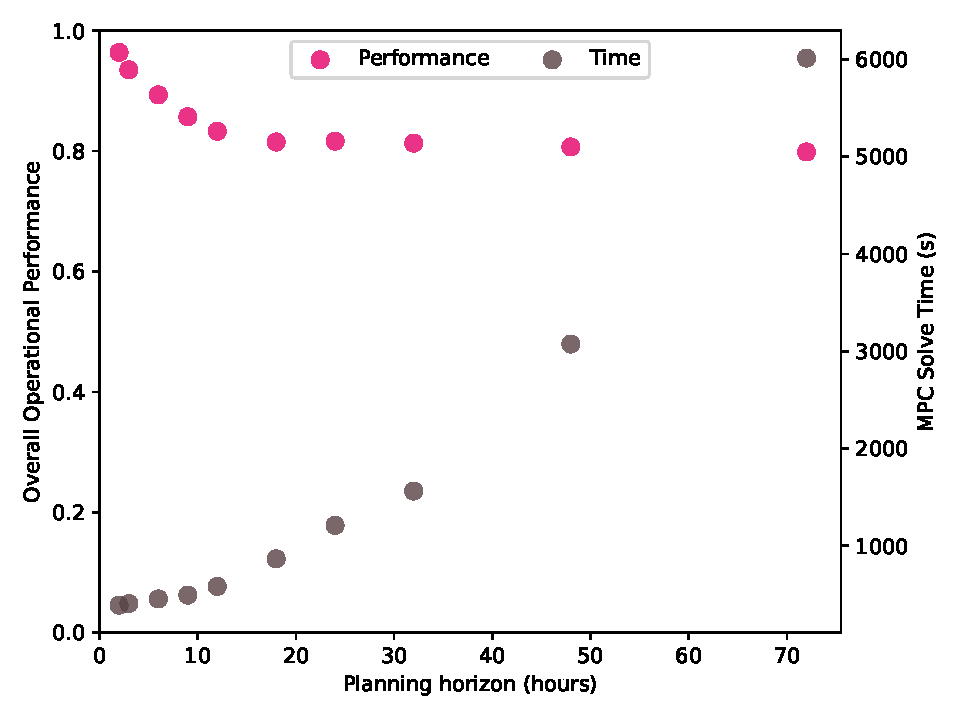
\includegraphics[width=0.6\linewidth]{Appendices/planning_horizon.pdf}
        \caption{Variation of perfect forecast \glsxtrshort{mpc} operational performance and computation time with planning horizon, $T$.}
        \label{fig:forecasting-planning-horizon}
    \end{figure}


    \newpage
    \section{Technical specification of prediction models and training procedures} \label{app:forecasting-models}

    % Provide references to package documentation for model implementations and training procedure.

    The model parameters and training procedure used for machine learning models have a significant impact on their performance, as well as their computational and data requirements. Hence, they must be selected carefully for the target application to maximise model performance with the available computational resources and data.

    \subsection{Simple neural models}

    For the simple neural models, implementations from the Pytorch Lighting library \citep{falcon2019PyTorchLightning} were used. The models use an input window of 168 time steps (input dimension) and output a forecast of 48 time steps (output dimension). All models were trained using the Adam optimizer \citep{kingma2017AdamMethodStochastic}, with a batch size of 32 and a learning rate determined using the built-in learning rate tuner.

    The Linear model consists of a single linear layer, of size 48, with no activation function used.

    The Convolution model uses two 1D convolution layers with channels (5, 1) and kernel sizes (5, 6), respectively, with ReLU activation functions. This is followed by an output MLP that brings the dimensionality to 48.

    The ResMLP model has an linear layer with 168 nodes, using a residual connection and ReLU activation. A subsequent output linear layer brings the dimensionality to 48.

    \subsection{State-of-the-art machine learning models}

    For the complex, state-of-the-art models, implementations from the Pytorch Forecasting library \citep{beitner2024Jdb78Pytorchforecasting} were used. The models take in data from the previous 72 time steps along with known covariate data from the coming 48 time steps, and output forecasts of the target variable for the coming 48 time steps. All models were trained using an early stopping trainer with a patience of 5, for a maximum of 50 epochs, with a limit of 800 training batches per epoch. The learning rate was determined using the built-in learning rate tuner. The size parameters, loss functions, and optimizers used are detailed in Table \ref{tab:complex-model-specs}.

    \begin{table}[h]
        \centering
        \renewcommand{\arraystretch}{1}
        \begin{tabularx}{\linewidth}{c|*{3}{>{\setlength{\baselineskip}{.5\baselineskip}}Y}} \toprule \toprule
            Model & TFT & NHiTS & DeepAR \\ \midrule
            Hidden size & 48 & 128 & 64 \\
            Drop-out & 0.1 & 0.1 & 0.1 \\
            Loss & Quantile loss & Quantile loss & Normal distribution loss \\
            Optimizer & Adam & AdamW & Adam \\[1ex]
            & \makecell{Attention head size: 4}
            & \makecell{Weight decay: 0.01\\Backcast loss ratio: 0}
            & \makecell{RNN layers: 3} \\
            \bottomrule\bottomrule
        \end{tabularx}
        \smallskip
        \caption{Technical specifications of complex, state-of-the-art models.}
        \label{tab:complex-model-specs}
    \end{table}


    \newpage
    \vspace*{0cm}
    \section{Data similarity metric} \label{app:forecasting-similarity-metric}

    \subsection{Functional data analysis}

    Functional Data Analysis (FDA) is used to analyse and compare the energy usage behaviours across the building electrical load dataset of 15 buildings. In this approach, functional principal components (fPCs) are extracted from the data, such that each data sample can be constructed from an equation of the form,

    \begin{equation}
        f(t) = \mu(t) + \sum_{i=1}^n \alpha_i \nu_i(t)
    \end{equation}

    i.e. the data sample, $f(t)$, is constructed from a linear sum of a mean function, $\mu(t)$, and a weighted sum of $n$ fPCs , $\nu_i(t)$, with weightings or `scores' $\alpha_i$. The mean function and fPCs are the same across all data samples, whereas the weightings are unique to each data sample. This has the benefit that to compare data samples, which are functions of time, it suffices to compare the weightings, a low-dimensional representation of the functional data, that can be analysed using standard statistical techniques.

    For this analysis, the datasets are pre-processed into daily time histories, such that each data sample is a 24 hour profile of electricity consumption, starting at midnight. For each building, the training dataset comprises 6 years of data and hence 2191 data samples, and the validation and test datasets are both 2 years and hence 731 and 730 data samples respectively (2016 was a leap year).

    The functional Principal Component Analysis (fPCA) approach used involves first aligning the data samples to a common mean, $\mu(t)$. This generates a warping function and an amplitude function for each data sample that describe how the data sample maps to the mean function. The warping function describes the phase relationship, i.e. the variation in time, and the amplitude function describes changes in magnitude. The warping and amplitude functions are then analysed separately and fPCs generated for both. The approach is illustrated schematically in Fig. \ref{fig:forecasting-fPCA-method}, and full details of the approach are described in (Ward, 2021) \citep{ward2021DatacentricStochasticModel}.

    Fig. \ref{fig:forecasting-fPC-effects} illustrates the first two phase and amplitude fPCs extracted from the dataset. Fig. \ref{fig:forecasting-fPCs-scatter} shows distributions of example fPC coefficients for Buildings 38 and 49. The load data for Building 49 exhibits a much lower range than that for Building 38, which results in a more positive distribution of V1 fPC coefficients. In Fig. \ref{fig:forecasting-fPC-effects} positive coefficients V1 fPC can be seen to reduce the data range.

    \begin{figure}[p]
        \centering
        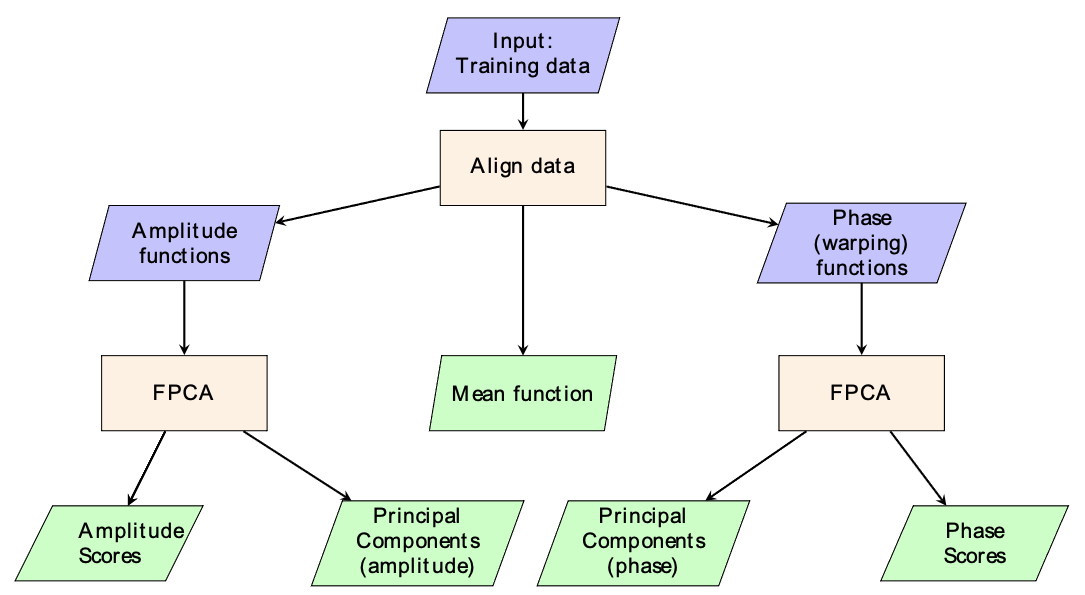
\includegraphics[width=0.6\linewidth]{Data_Analysis/fPCA-flow-diag.png}
        \caption{Schematic process for functional principal component analysis (fPCA)}
        \label{fig:forecasting-fPCA-method}
    \end{figure}

    \begin{figure}[p]
        \centering
        \begin{minipage}{.525\textwidth}
            \centering
            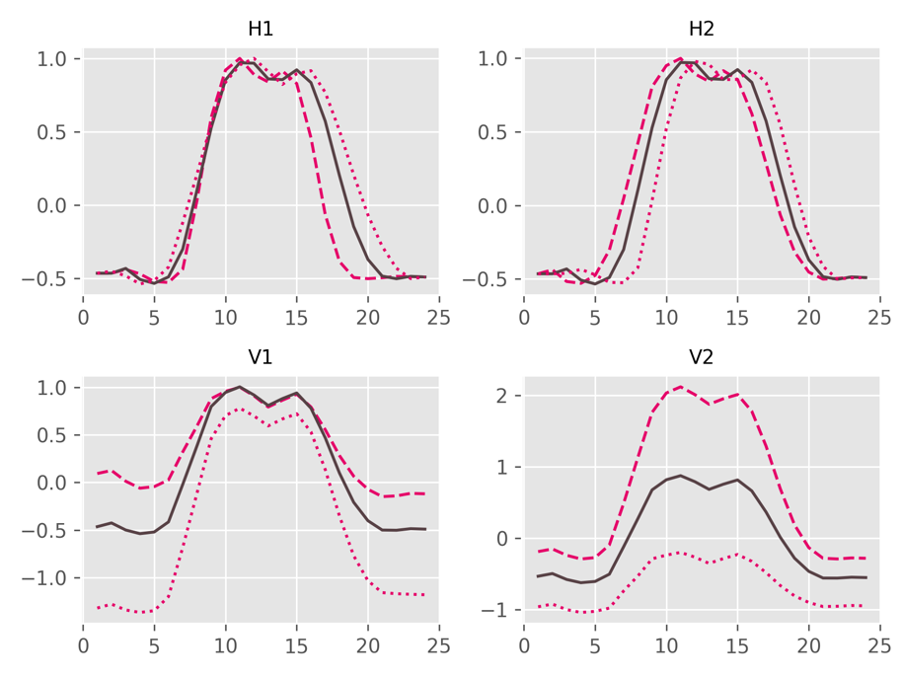
\includegraphics[width=0.9\linewidth]{Data_Analysis/fPC-effects.png}
            \caption{Illustration of first two Phase (H) and Amplitude (V) fPCs. Solid black line shows mean function, $\mu(t)$. Dashed line (-) indicates the impact of a +ve coefficient and dotted line (.), a -ve coefficient.}
            \label{fig:forecasting-fPC-effects}
        \end{minipage}%
        \hfill
        \begin{minipage}{.425\textwidth}
            \centering
            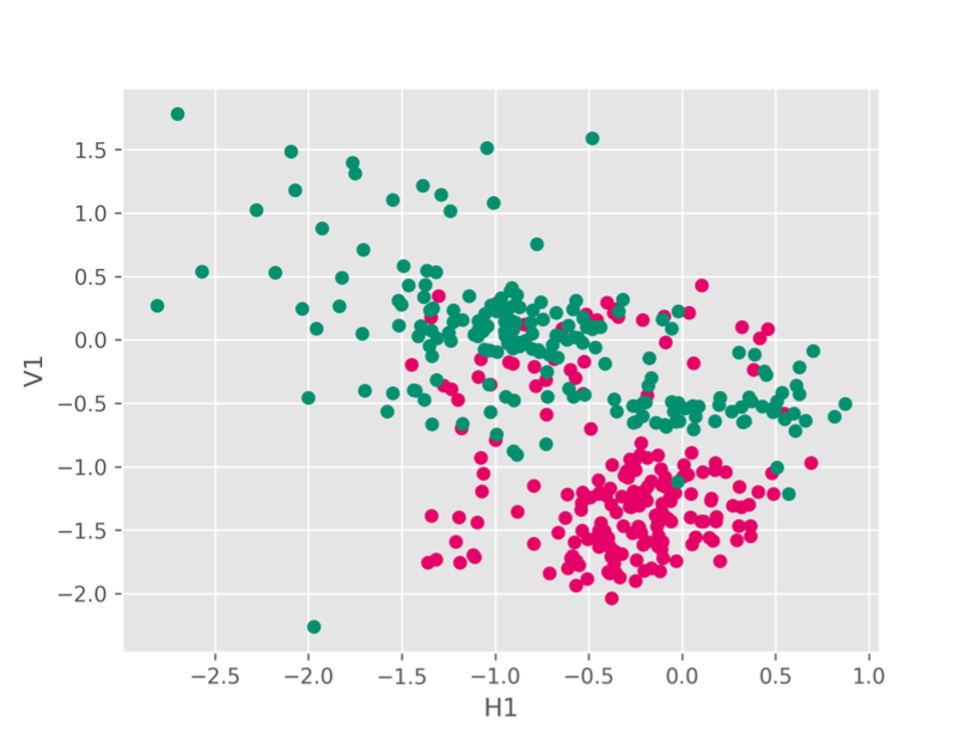
\includegraphics[width=\linewidth]{Data_Analysis/fPC-scatter.png}
            \caption{Example fPC coefficient distributions for Buildings 38 (pink) and 49 (green)}
        \label{fig:forecasting-fPCs-scatter}
        \end{minipage}%
    \end{figure}

    % Move here to get data analysis figures on a page
    \begin{figure}[p]
        \centering
        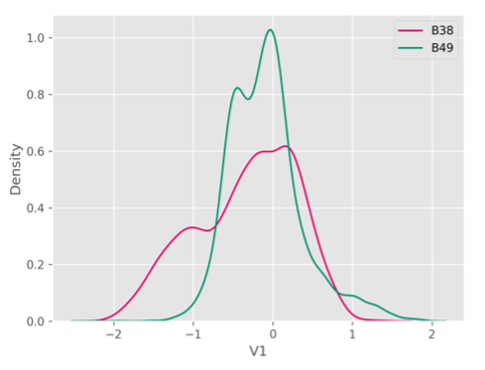
\includegraphics[width=0.4\linewidth]{Data_Analysis/fPC-dist-comparison.png}
        \caption{Kernel density plot of V1 scores for Buildings 38 \& 49. Wasserstein distance between two distributions is 0.05.}
        \label{fig:forecasting-fPC-comparison}
    \end{figure}

    \subsection{Wasserstein similarity metric} \label{forecasting-similarity-metrics}

    The deconstruction of the data into fPCs and corresponding coefficients enables the use of standard statistical techniques to define measures of similarity between load profiles in the dataset. A load profile similarity metric based on an optimal transport approach is proposed. This metric is based on the approximate Wasserstein distance, or Earth-mover's distance, between the distributions of PC coefficients, which provides a measure of the ease with which one probability distribution can be transformed into the other, and hence is a measure of the similarity of the two distributions. As such, the metric is referred to as the `Wasserstein similarity metric', and is computed using the \href{https://github.com/jeanfeydy/geomloss}{Geomloss} \citep{feydy2024JeanfeydyGeomloss} library. Advantages of this method are that it provides a comparison of the underlying patterns in the load profiles that is not excessively distorted by sequence misalignments as is the case for simple metrics like RMSE, and it allows time series of different durations to be compared.

    % Q: what's approximate about the calculation? A: It's a complex calculation and the methodology purports to give an approximate solution
    % Q: What specifically is the metric? The average Wasserstein distance over all fPCs? A: It is the distance between one multivariate distribution and another.  So it is the distance between sets of PC coefficients.  

    Fig. \ref{fig:forecasting-fPC-comparison} shows the kernel density distributions of the V1 fPC coefficients for Buildings 38 and 49. The Wasserstein distance between these distributions is 0.05. Similarity metric values are computed for comparison of the training datasets between pairs of buildings, and for the comparison of pairs of training, validation, and test datasets for each building individually. Figures \ref{fig:forecasting-similarities-buildings} \& \ref{fig:forecasting-similarities-datasets} provide the results of these similarity metric calculations.

    \begin{figure}
        \centering
        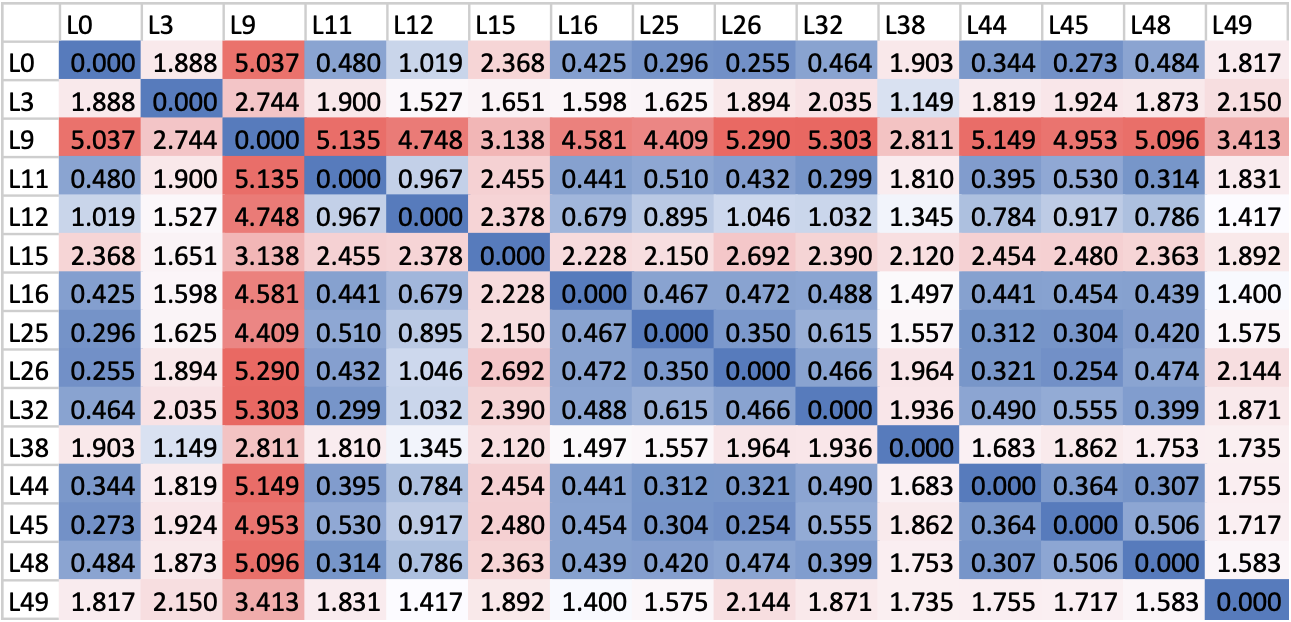
\includegraphics[width=0.8\linewidth]{Data_Analysis/building-similarities.png}
        \caption{Similarity metric scores between training datasets for pairs of buildings.}
        \label{fig:forecasting-similarities-buildings}
    \end{figure}

    \begin{figure}
        \centering
        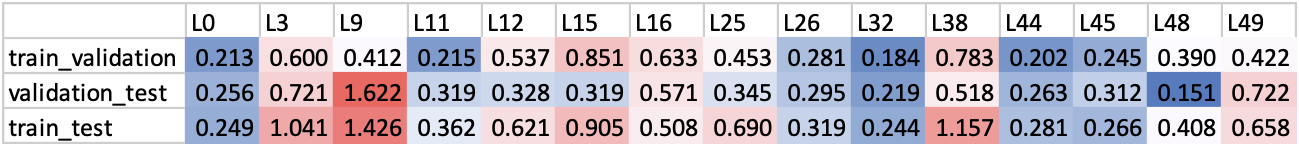
\includegraphics[width=0.8\linewidth]{Data_Analysis/data-similarities.png}
        \caption{Similarity metric scores between pairs of training, validation, test datasets for each building.}
        \label{fig:forecasting-similarities-datasets}
    \end{figure}

    % A similarity metric is proposed to enable the efficient comparison of load profiles.
    % The potential of this metric to provide a data analysis based methodology for estimating prediction model generalisation performance is investigated in Section 7.


    \newpage
    \vspace*{0cm} % classic tex jank
    \section{Change-point analysis} \label{app:forecasting-change-points}

    Building electrical loads are driven by occupancy behaviour dynamics which span timescales: seasonal (winter heating vs. summer cooling loads), weekly (inhabitance trends due to working patterns, i.e. weekday vs. weekend), and daily (nighttime vs. daytime). The form of these behavioural trends also differs between buildings depending on their usage, e.g. offices and residential buildings have opposing daily trends. Gradual changes can occur in these behavioural trends, for instance due to cultural shifts in working patterns. Alternatively, abrupt changes can be caused by severe disturbances, such as building stock refurbishment, temporary vacancy, or occupant behavioural changes due to change in building use. As such, changes can occur in the seasonal and/or trend patterns of building load time series, and the underlying patterns of the dynamics can differ significantly following disturbances.

    This raises the question as to whether all historic measurement data is useful for the training of load prediction models, as the underlying patterns in certain sections of the historic data may differ significantly from the current behaviour of the building load, i.e. be non-representative. Including these sections in the training dataset may poison model training, leading to worse prediction performance.

    \begin{figure}[t]
        \centering
        \hspace*{\fill}
        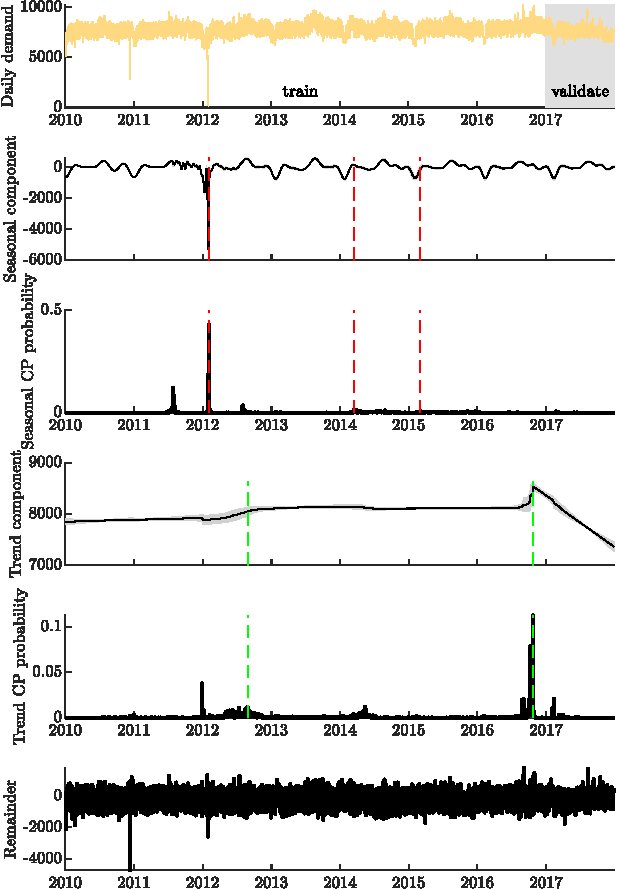
\includegraphics[width=0.45\linewidth]{Changepoint/Annexe37_CPoutput_B26_eps-conv.pdf}
        \hspace*{\fill}
        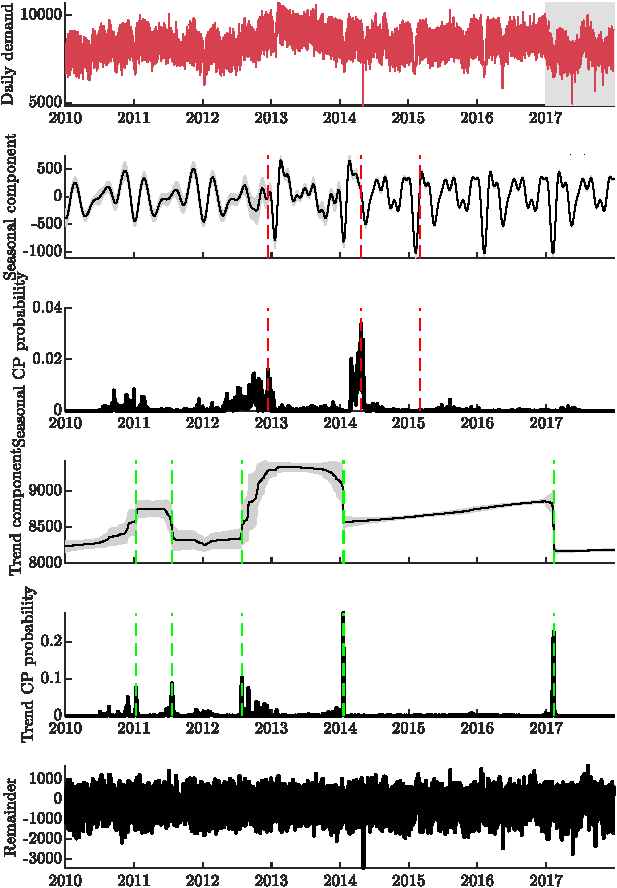
\includegraphics[width=0.45\linewidth]{Changepoint/Annexe37_CPoutput_B44_eps-conv.pdf}
        \hspace*{\fill}
        \bigskip
        \caption{Change-points detected using the BEAST algorithm in load profiles of Buildings 26 \& 44 (top row). Signal is decomposed into a seasonal component (second row), assumed harmonic, inferred change-points indicated by red vertical lines, and a trend component (fourth row), with green lines indicating change-points. Credible intervals of the estimated signals are given by grey envelopes around the individual components.}
        \label{fig:forecasting-change-points}
    \end{figure}

    A change-point analysis is conducted on the building electrical load dataset to detect changes in the load patterns in each building. The Bayesian ensemble algorithm ``Bayesian Estimator of Abrupt change, Seasonal change, and Trend'' (BEAST) \citep{zhao2019DetectingChangepointTrend} is used to decompose the load time series and derive non-linear dynamics across multiple timescales, detecting change-points, seasonality, and trends. The value of this ensemble approach is that it quantifies the relative usefulness of individual decomposition models, leveraging all the models via Bayesian model averaging. Additionally, it provides an estimated probability of inferred change-points being `true’ change-points. Results of the change-point analysis for Buildings 26 \& 44 are shown in Fig. \ref{fig:forecasting-change-points}. The demand profiles are decomposed into seasonal and trend components, and detected change-points for the two components are indicated in red and green respectively. The trend component of Building 44 is found to vary substantially more than that of Building 26, which corresponds with the visual variability of the demand profiles.
\end{subappendices}